% ===============================================
% Graduate Project 2026 -- companion paper
% paper.tex
% Same basic format as docs/presentation/main.tex
% ===============================================

\documentclass[11pt]{article}

\usepackage[margin=1in]{geometry}
\usepackage[T1]{fontenc}
\usepackage{lmodern}
\usepackage{microtype}   % finer spacing and line breaking
\usepackage{amsmath,amsthm,amssymb}
\usepackage{enumitem}
\usepackage{graphicx}
\usepackage{tikz}
\usepackage{parskip}
\usepackage{booktabs}
\usepackage{needspace}   % keeps the Acknowledgments from splitting across pages
\usepackage{placeins}   % \FloatBarrier keeps a float from drifting into the next subsection
\usepackage{xurl}   % lets long URLs in the bibliography break
\usepackage[style=authoryear-comp,maxcitenames=2,uniquelist=false,backend=bibtex,dashed=false]{biblatex}
\addbibresource{../lit_review/references.bib}
\AtEveryBibitem{\clearfield{note}}   % provenance notes stay in references.bib, not in the printed list
\setcounter{biburlnumpenalty}{100}\setcounter{biburlucpenalty}{100}\setcounter{biburllcpenalty}{100}   % let long URLs break
\usepackage[hidelinks,bookmarksnumbered]{hyperref}   % clickable refs, cites, URLs; numbered PDF bookmarks
\hypersetup{pdftitle={Traversing the Unlikely Intersection of Topological Data Analysis's Mapper Algorithm and Pitch-Level MLB Data}, pdfauthor={Will Paz}, pdfkeywords={topological data analysis, Mapper, persistent homology, baseball, pitch classification}}

% GENERATED by src/viz/paper_numbers.py -- do not edit by hand
\newcommand{\NPitches}{721{,}799}
\newcommand{\NPitchesTwentySix}{727{,}721}
\newcommand{\NShapes}{3{,}943}
\newcommand{\NFeatures}{9}
\newcommand{\NNodes}{66}
\newcommand{\NEdges}{143}
\newcommand{\NComponents}{9}
\newcommand{\GiantShapes}{3{,}273}
\newcommand{\NSlowComps}{five}
\newcommand{\NOtherComps}{three}
\newcommand{\NoiseShapes}{630}
\newcommand{\PCone}{38.5}
\newcommand{\PCtwo}{21.0}
\newcommand{\PCASixPct}{95.5}
\newcommand{\GraphBone}{86}
\newcommand{\NerveBone}{1}
\newcommand{\NerveRank}{85}
\newcommand{\StuffTrainN}{2{,}008{,}693}
\newcommand{\GridGraphBoneMin}{33}
\newcommand{\GridGraphBoneMax}{147}
\newcommand{\GridNerveBoneMin}{0}
\newcommand{\GridNerveBoneMax}{4}
\newcommand{\DimMLE}{6.26}
\newcommand{\DimTwoNN}{6.76}
\newcommand{\DimNullMLE}{7.07}
\newcommand{\PeakBB}{0.17}
\newcommand{\PeakCH}{0.08}
\newcommand{\LSTwentyFiveBoundary}{168}
\newcommand{\LSTwentyFiveEligible}{1{,}525}
\newcommand{\LSTwentyFiveBoundaryPct}{11}
\newcommand{\LSTwentyFiveShift}{11.5}
\newcommand{\LSTwentyFiveOneSDPct}{38}
\newcommand{\LSTwentyFiveTwoSEPct}{96}
\newcommand{\LSTwentyFiveCrossPct}{32}
\newcommand{\LSTwentyFivePctChange}{17}
\newcommand{\LSTwentySixBoundary}{150}
\newcommand{\LSTwentySixEligible}{1{,}565}
\newcommand{\LSTwentySixBoundaryPct}{10}
\newcommand{\LSTwentySixShift}{9.2}
\newcommand{\LSTwentySixOneSDPct}{33}
\newcommand{\LSTwentySixTwoSEPct}{93}
\newcommand{\LSTwentySixCrossPct}{25}
\newcommand{\LSTwentySixPctChange}{17}
\newcommand{\DevN}{1{,}876}
\newcommand{\DevBetterBeta}{0.06}
\newcommand{\DevBetterLo}{\ensuremath{-}0.09}
\newcommand{\DevBetterHi}{0.22}
\newcommand{\DevBetterP}{0.421}
\newcommand{\DevRandomBeta}{\ensuremath{-}0.20}
\newcommand{\DevRandomLo}{\ensuremath{-}0.36}
\newcommand{\DevRandomHi}{\ensuremath{-}0.03}
\newcommand{\DevRandomP}{0.020}
\newcommand{\DevWorseBeta}{\ensuremath{-}0.25}
\newcommand{\DevWorseLo}{\ensuremath{-}0.44}
\newcommand{\DevWorseHi}{\ensuremath{-}0.07}
\newcommand{\DevWorseP}{0.006}
\newcommand{\DevExRandomBeta}{\ensuremath{-}0.26}
\newcommand{\DevExRandomP}{0.005}
\newcommand{\DevExBetterBeta}{0.17}
\newcommand{\DevExBetterP}{0.063}
\newcommand{\TypN}{3{,}114}
\newcommand{\TypBeta}{\ensuremath{-}0.59}
\newcommand{\TypLo}{\ensuremath{-}0.81}
\newcommand{\TypHi}{\ensuremath{-}0.37}
\newcommand{\TypSecBeta}{\ensuremath{-}0.18}
\newcommand{\TypSecP}{0.09}
\newcommand{\YoungPlanned}{87}
\newcommand{\YoungClear}{3}
\newcommand{\JumpAge}{23}
\newcommand{\JumpN}{398}
\newcommand{\JumpGainOne}{0.93}
\newcommand{\JumpGainEnd}{2.03}
\newcommand{\JumpEndSeason}{3}
\newcommand{\JumpSweepStart}{5.1}
\newcommand{\JumpSweepOne}{2.3}
\newcommand{\JumpSweepEnd}{0.1}
\newcommand{\NPitchesTwentyFour}{745{,}350}
\newcommand{\NPitchesTwentyThree}{732{,}562}
\newcommand{\MedianPitches}{98}
\newcommand{\PctLtFive}{9}
\newcommand{\PctLtTwenty}{22}
\newcommand{\NSlow}{131}
\newcommand{\SlowMedian}{9}
\newcommand{\SlowQ}{2}
\newcommand{\SSOneShapes}{3{,}942}
\newcommand{\SSOneSlow}{131}
\newcommand{\SSOneComp}{8}
\newcommand{\SSOneIso}{97\%}
\newcommand{\SSOneRho}{1.00}
\newcommand{\SSTenShapes}{3{,}391}
\newcommand{\SSTenSlow}{63}
\newcommand{\SSTenComp}{6}
\newcommand{\SSTenIso}{89\%}
\newcommand{\SSTenRho}{1.00}
\newcommand{\SSTwentyShapes}{3{,}073}
\newcommand{\SSTwentySlow}{29}
\newcommand{\SSTwentyComp}{8}
\newcommand{\SSTwentyIso}{none in a node}
\newcommand{\SSTwentyRho}{0.98}
\newcommand{\StabOrderMin}{100}
\newcommand{\StabSlowPCALo}{97}
\newcommand{\StabSlowPCAHi}{100}
\newcommand{\StabSlowLo}{94}
\newcommand{\StabSlowHi}{100}
\newcommand{\NullOrderMin}{100}
\newcommand{\NullSlowLo}{50}
\newcommand{\NullSlowHi}{78}
\newcommand{\GaussGraphBoneMin}{56}
\newcommand{\GaussGraphBoneMax}{97}
\newcommand{\GaussNerveBoneMin}{2}
\newcommand{\GaussNerveBoneMax}{9}
\newcommand{\ShuffleGraphBoneMin}{56}
\newcommand{\ShuffleGraphBoneMax}{80}
\newcommand{\ShuffleNerveBoneMin}{0}
\newcommand{\ShuffleNerveBoneMax}{2}
\newcommand{\PHRealLoops}{0}
\newcommand{\PHRealLongBars}{17}
\newcommand{\PHLongSingles}{11}
\newcommand{\PHLongMaxGroup}{7}
\newcommand{\PHGaussLongBarsLo}{17}
\newcommand{\PHGaussLongBarsHi}{23}
\newcommand{\PHShuffleLongBarsLo}{57}
\newcommand{\PHShuffleLongBarsHi}{64}
\newcommand{\PHRealHzeroMedian}{1.00}
\newcommand{\PHGaussHzeroMedian}{1.53}
\newcommand{\DimNullTwoNN}{7.52}
\newcommand{\DimTypeGapLo}{0.4}
\newcommand{\DimTypeGapHi}{1.2}
\newcommand{\PeakCurve}{0.013}
\newcommand{\PeakSweep}{0.012}
\newcommand{\PeakP}{0.02}
\newcommand{\PCPeaks}{2}
\newcommand{\PCBandLo}{0.15}
\newcommand{\PCBandHi}{0.30}
\newcommand{\MultiTwentyFive}{55}
\newcommand{\MultiTwentySix}{55}
\newcommand{\OmegaWhiffLabels}{2.8}
\newcommand{\OmegaWhiffCentroid}{1.9}
\newcommand{\OmegaWhiffMapper}{1.5}
\newcommand{\OmegaGBLabels}{3.4}
\newcommand{\OmegaGBCentroid}{1.8}
\newcommand{\OmegaGBMapper}{0.9}
\newcommand{\ReliabilityRho}{\ensuremath{-}0.78}
\newcommand{\FlComp}{1}
\newcommand{\FlGraphBone}{139}
\newcommand{\FlNerveBone}{0}
\newcommand{\FlGridCompMax}{2}
\newcommand{\FlGridNerveMin}{0}
\newcommand{\FlGridNerveMax}{5}
\newcommand{\FlNullNerveMin}{0}
\newcommand{\FlNullNerveMax}{2}
\newcommand{\FlSlowIso}{0}
\newcommand{\FlLongBars}{99}
\newcommand{\FlGaussLongBarsLo}{476}
\newcommand{\FlGaussLongBarsHi}{519}
\newcommand{\FlDimMLE}{4.40}
\newcommand{\FlDimNullMLE}{4.78}
\newcommand{\FlRuns}{8}
\newcommand{\FlAllNerveMax}{6}
\newcommand{\FlAllSlowIso}{0}
\newcommand{\FlSixLongBars}{100}
\newcommand{\FlSixLoops}{0}
\newcommand{\FlSixGaussLo}{489}
\newcommand{\FlSixGaussHi}{539}
\newcommand{\FlSixDim}{4.33}
\newcommand{\FlSixDimNull}{4.77}
\newcommand{\FlSixComp}{1}
\newcommand{\FlSixGridCompMax}{4}
\newcommand{\FlSixGridNerveMin}{0}
\newcommand{\FlSixGridNerveMax}{4}
\newcommand{\FlSixNullNerveMin}{0}
\newcommand{\FlSixNullNerveMax}{3}
\newcommand{\FlSixSlowIso}{0}
\newcommand{\NullNerveBoneMin}{0}
\newcommand{\NullNerveBoneMax}{9}
\newcommand{\LSPairFCSL}{45}
\newcommand{\LSPairCHFS}{37}
\newcommand{\LSPairCUKC}{23}
\newcommand{\LSPairSLST}{15}
\newcommand{\LSPairFCFF}{9}
\newcommand{\JansenNbFF}{18}
\newcommand{\JansenOwnGrade}{86}
\newcommand{\JansenAltGrade}{106}
\newcommand{\BandBoundaryIn}{30}
\newcommand{\BandBoundaryN}{44}
\newcommand{\BandAllPct}{51}
\newcommand{\BandBoundaryPct}{68}
\newcommand{\ExOwnName}{knuckle curve}
\newcommand{\ExAltName}{curveball}
\newcommand{\ExOwnGrade}{97}
\newcommand{\ExAltGrade}{109}
\newcommand{\ExNbOwn}{3}
\newcommand{\ExNbAlt}{16}
\newcommand{\DesignNeighbors}{10}
\newcommand{\DesignSwStr}{4.9}
\newcommand{\DesignNbSwStr}{7.6}
\newcommand{\DesignIVBGain}{1.7}
\newcommand{\CircNullGraphBoneMax}{0}
\newcommand{\CircNullCompLo}{2}
\newcommand{\CircNullCompHi}{8}
\newcommand{\RipsBirth}{0.625}
\newcommand{\RipsDeath}{1.617}
\newcommand{\RipsPers}{0.992}
\newcommand{\RipsNext}{0.005}
\newcommand{\PHMaxPers}{0.87}
\newcommand{\PHGaussMaxPersLo}{0.75}
\newcommand{\PHGaussMaxPersHi}{0.88}
\newcommand{\FlMaxPers}{2.02}
\newcommand{\FlGaussMaxPersLo}{1.55}
\newcommand{\FlGaussMaxPersHi}{1.85}
\newcommand{\FlSixMaxPers}{2.04}
\newcommand{\FlSixGaussMaxPersLo}{1.60}
\newcommand{\FlSixGaussMaxPersHi}{1.99}
   % GENERATED by src/viz/paper_numbers.py: every reported number

\newcommand{\R}{\mathbb{R}}
\newcommand{\Z}{\mathbb{Z}}
\newcommand{\N}{\mathbb{N}}
\DeclareMathOperator{\rank}{rank}
\DeclareMathOperator{\diam}{diam}
\graphicspath{{../presentation/figures/}}

% Drafting aids (plain text, no colors).
% \pendingcite: a source not yet through the citation ledger; prints [key?].
% \plan: what a section will contain and where it comes from; prints as an
% italic note. Set \showplanfalse to hide all plans.
\newcommand{\pendingcite}[1]{[#1?]}
\newif\ifshowplan \showplanfalse
\newcommand{\plan}[1]{\ifshowplan\par\emph{[Plan: #1]}\par\fi}

\newtheorem{theorem}{Theorem}[section]
\newtheorem{lemma}[theorem]{Lemma}
\newtheorem{proposition}[theorem]{Proposition}
\newtheorem{corollary}[theorem]{Corollary}
\theoremstyle{definition}
\newtheorem{definition}[theorem]{Definition}
\newtheorem{example}[theorem]{Example}
\theoremstyle{remark}
\newtheorem{remark}[theorem]{Remark}

% Alternative title stating the finding:
% "Pitch Labels Cut a Connected Space: Certifying Mapper on MLB Pitch Shapes"
\title{Traversing the Unlikely Intersection of Topological Data Analysis's Mapper Algorithm and Pitch-Level MLB Data}
\author{Will Paz\\ Miami University\\ \texttt{pazwj@miamioh.edu}}
\date{\today}

\begin{document}
\maketitle

\begin{abstract}
In every Major League Baseball game, pitch-tracking systems capture a multitude of physical characteristics, such as spin rate, velocity, and movement, that can help classify and label any given pitch thrown.
But due to the continuous nature of these measurements, classifying pitches such as sliders and cutters, or changeups and splitters, can become incredibly challenging.
In this paper, we explore whether these pitch labels indicate separate groups or divide one connected space, as well as the mathematical foundation that lies within the methodology used.
Given the \NShapes{} per-pitcher, per-pitch-type averages of eight Statcast measurements (nine coordinates) from the 2025 season, we use the Mapper algorithm from topological data analysis and test each feature that Mapper shows against covariance-matched null models and against invariants that do not depend on Mapper at all.
We find that pitch shapes create one connected continuum apart from slow outlier pitches, with no gaps or loops beyond those of a Gaussian with the same covariance.
At the individual pitch level, the density has three robust peaks: fastballs, breaking balls, and offspeed pitches.
The \GraphBone{} loops in the Mapper graph come from reading only its 1-skeleton; the full nerve has only \NerveBone.
With the current labeling system, analyzing and grading a pitch within its own label is fragile for roughly a tenth of the pitch shapes with enough pitches to test, the ones that sit near a label boundary.
Ultimately, we see this work as groundwork. A continuum view could open new ways of grading pitches and developing pitchers, and we leave those ideas to future work.
\end{abstract}
\noindent\textbf{Keywords:} topological data analysis, Mapper, persistent homology, baseball, pitch classification

%======================================================================
\section{Introduction}
%======================================================================
Let us start with a simple question.
Where does red end and orange begin?
You can point to a red and to an orange, but somewhere between them there is a color that two people would name differently.
The reason for this is that the colors themselves run continuously, and the names are just lines that we draw across them.
The same question can be posed for pitch types in baseball.
A slider and a cutter can come out of a pitcher's hand at nearly the same speed and move in nearly the same way, yet one is compared with sliders and the other with cutters.
Every pitch thrown in a Major League game is tracked, with its velocity, movement, spin, and release recorded \parencite{savantcsvdocs}, and it is given a label, such as four-seam fastball, sinker, cutter, slider, sweeper, curveball, or changeup \parencite{mlbglossary_pitchtypes}.
These labels are used across all facets of baseball, from scouting and player development to in-game strategy and analytics.

Our goal is to explore the geometry of pitch shapes, to understand how the labels relate to that geometry, and ultimately to ask whether the labels are meaningful in a geometric sense.
Do pitch shapes fall into separate clumps, so that each label names its own group?
Do they create one connected space that the labels simply divide?
Or is the answer somewhere in between, with a connected space that has a few dense regions?
Topological data analysis is built for questions of this kind, and in our case we focus on its Mapper algorithm, introduced by Singh, M\'emoli, and Carlsson in 2007 \parencite{singh2007mapper}, which produces a graph summary of a point cloud that is quite readable.
But just as the Mapper graph is easy to read, it is also easy to over-read, since it can show structure that the covariance of the data alone produces \parencite{topaz2026null}, and its loops can be artifacts of the construction itself (Section~\ref{sec:loops}).

When we first ran Mapper on the \NShapes{} pitch shapes from the 2025 season, the graph gave us \GraphBone{} loops, and a real loop would have been a discovery, since it would mean a ring of pitch shapes circling a hole, a mix of velocity, movement, and spin that no pitcher throws.
Unfortunately, they are not real.
Once we fill in the triangles that the graph leaves out, the full nerve of the cover keeps only \NerveBone{} loop, and every other test we ran found no holes or gaps beyond what our null models produce.
What we found instead is the in-between answer.
Apart from the slowest, outlier pitches, we can walk from a curveball to a four-seam fastball one small step at a time, through shapes that other pitchers actually throw, without ever crossing a gap.
Along the way, single pitches crowd into three dense regions, those being the fastballs, breaking balls, and offspeed pitches that anyone who follows baseball already knows, which matches what \textcite{maloof2026classify} found for college pitches.
The finer names are simply the lines we draw across this continuum, and the Mapper graph shows where at least one of them falls, in a band of sliders and cutters between the breaking balls and the fastballs.

This continuum matters for baseball, since pitches are graded against their labels.
For example, Kenley Jansen's cutter grades \JansenOwnGrade{} among cutters but \JansenAltGrade{} among four-seamers, the pitches it most resembles, so whether it counts as below or above average depends on where the label line falls.
Jansen's cutter is not alone.
When a pitch is graded within its own label, whether on the per-type scale of a Stuff+-style model or through an ``elite among sliders'' percentile, the grade is fragile for the \LSTwentyFiveBoundaryPct\% of testable pitch shapes that sit near a label boundary.
For those pitches, relabeling moves the grade by a median of \LSTwentyFiveShift{} points in 2025 and \LSTwentySixShift{} in 2026, on a scale with a standard deviation of 15, and in seasons that our models never saw.
From there, we look at what thinking of pitches as a continuum could offer, from pitch design and player development to new ways of labeling and grading pitches, which we leave as ideas for future work rather than results.

We wrote this paper with two readers in mind, a mathematician who may not know a slider from a cutter and a baseball reader who may not know a simplicial complex.
In order to serve both, we begin with background on how pitches are measured, labeled, and graded (Section~\ref{sec:background}).
Sections~\ref{sec:topology} and~\ref{sec:mapper} then cover the topology that we need as well as the Mapper algorithm, with small examples along the way.
Next, Section~\ref{sec:data} describes the data, Section~\ref{sec:certify} the methods that we use to test what Mapper shows, Section~\ref{sec:shape} the shape results, and Section~\ref{sec:consequences} the consequences for pitch evaluation and design.
We finish with a discussion in Section~\ref{sec:discussion}, where we compare our results with prior work and go over limitations and future studies.
The code and data products used in this work are available on GitHub (Appendix~\ref{app:repro}).

%======================================================================
\section{Background}\label{sec:background}
%======================================================================
\subsection{Statcast}\label{sec:statcast}
Introduced in 2015, Statcast is a pitch-tracking system that, since 2020, uses high-speed cameras to measure a variety of useful data points for every pitch thrown in a Major League Baseball game \parencite{mlbglossary_statcast}.
For our purposes, we will focus on the physical characteristics of a given pitch, which include the velocity, movement, spin, and release of the pitch, amongst others.

To define which of these characteristics we will use, we will first describe how Statcast measures each pitch and what each measurement means.
For each pitch it records the velocity out of the hand in miles per hour, the horizontal and vertical movement $\mathit{pfx}_x$ and $\mathit{pfx}_z$ in feet from the catcher's view, the spin rate in revolutions per minute, the spin axis, and the release point and release extension in feet \parencite{savantcsvdocs,mlbglossary_spinrate}.
Some of these may be intuitive, such as velocity, but others such as spin axis and release extension may require further explanation.
Horizontal movement is described relative to the pitcher, so when it is described as arm-side, the ball is moving toward the side of the pitcher's throwing arm, and conversely, glove-side movement moves toward the other side \parencite{savantcsvdocs,mlbglossary_slurve}.
The other baseball adjustment to this data is that vertical movement is usually reported as induced vertical break, which is the ride or drop that the pitcher creates with the effects of gravity removed \parencite{mlbglossary_ivb}.
Statcast documents $\mathit{pfx}_z$ only as vertical movement, so the fact that it excludes gravity, and is therefore induced vertical break, is our own inference from the data, since four-seam fastballs average about $+1$ foot.
Lastly, spin axis is an angle from $0^\circ$ to $360^\circ$, in which $180^\circ$ is pure backspin and $0^\circ$ pure topspin \parencite{savantcsvdocs}, while extension is a measure of how much closer to home plate than the pitching rubber the pitcher releases the ball \parencite{mlbglossary_extension}.

Each particular pitch also carries a Statcast pitch-type code, such as FF for a four-seam fastball, SI for a sinker, FC for a cutter, SL for a slider, ST for a sweeper, CU for a curveball, CH for a changeup, and FS for a splitter \parencite{mlbglossary_pitchtypes}.
For the purposes of this paper, we group these into three families, which are fastballs (FF, SI, FC), breaking balls (SL, ST, CU, and the rarer slurve SV, knuckle curve KC, and slow curve CS), and offspeed pitches (CH, FS, and the rare forkball FO), and this grouping into families is our own.
Some will call offspeed pitches changeups, but we will use the term offspeed to include splitters as well, for a cleaner naming convention.
There are a few other pitch types that are not included in these three families, such as the eephus, knuckleball, and screwball. They are rare, but they are still in our data, and the eephus pitches sit among the very slow pitches that come apart from the rest in Section~\ref{sec:shape}.
For readers unfamiliar with these pitches, I would encourage them to learn more about these unique pitch offerings. The eephus even has a film carrying its name, which I would highly recommend to the baseball fans out there \parencite{eephusfilm}.

\subsection{Pitch Classification}\label{sec:labels}
As the pitch-tracking era has progressed through the years in Major League Baseball, the methods of pitch classification have also evolved.
MLB describes its pitch-classification system as patented neural-network software, customized for every pitcher, that classifies nearly 750{,}000 pitches a season \parencite{sharpe2020classification}.
The underlying patent claims a method where a pitch is classified from its measured properties together with the pitch types previously determined to be in that pitcher's repertoire, and is then assigned the type most likely to match its trajectory \parencite{paul2014patent}.
Under this system, labels are assigned pitcher by pitcher, and a pitcher's own name for a pitch often comes from its grip or how it feels out of the hand, not only from how it moves, so the same physical shape can end up with different labels for different pitchers.
Other work has grouped pitches by their physics alone, without any labels, and we compare our results with that work in Section~\ref{sec:prior}.

\subsection{Pitch Grading}\label{sec:grading}
Alongside labeling and classifying pitches, teams and analysts also grade them.
Some pitch-quality models score a pitch only from its physical characteristics, such as FanGraphs' Stuff+ \parencite{mcgrattan2023stuffplus}.
Much of the methodology behind advanced Stuff+-style models is proprietary, but they all share the same goal of grading the quality of a pitch.
In this paper, we build our own Stuff+-style models (Section~\ref{sec:consequences}), which predict three outcomes of a pitch from its physical measurements, those being the quality of contact, measured by expected weighted on-base average (xwOBA), whether the batter swings and misses, and whether the batter chases a pitch outside the strike zone.
We then combine the three predictions into one grade on a scale with a mean of 100 and a standard deviation of 15.
A grade like this can be reported within a pitch type, comparing a slider only with other sliders, and Section~\ref{sec:labelfragile} shows why that choice is fragile for pitches near a label boundary.
The homemade Stuff+ model is not meant to be the focal point of this paper, but it is a useful tool for understanding the consequences of our shape results.

%======================================================================
\section{Topological Background}\label{sec:topology}
%======================================================================
Before we can describe Mapper, we ought to introduce the topology that lays its foundation.
As we progress in this section, we will state each definition in full and cite the theorems that we use without proving them.
Throughout this paper, every space will be a subset of some $\R^n$ with the topology induced by Euclidean distance, with the general notions of topological space and subspace topology being standard \parencite{munkres2000topology}.

\subsection{Homotopy}
\begin{definition}[Homotopy, {\cite{hatcher2001}}]
Continuous maps $f, g : X \to Y$ are \emph{homotopic}, written $f \simeq g$, if there is a continuous map $F : X \times [0,1] \to Y$ with $F(x,0) = f(x)$ and $F(x,1) = g(x)$ for all $x \in X$.
Spaces $X$ and $Y$ are \emph{homotopy equivalent}, $X \simeq Y$, if there are continuous maps $f : X \to Y$ and $g : Y \to X$ with $g \circ f \simeq \mathrm{id}_X$ and $f \circ g \simeq \mathrm{id}_Y$.
A space homotopy equivalent to a point is \emph{contractible}.
\end{definition}
For example, a disk is contractible, while a circle is not, and the boundary of a triangle is homotopy equivalent to a circle.
When we say that two spaces have the same shape, we mean that they are homotopy equivalent, which ignores size and distance but keeps track of pieces and loops, which we count with Betti numbers later in this section.

\subsection{Simplices and Simplicial Complexes}
\begin{definition}[Simplex, {\cite{hatcher2001}}]
Points $v_0, \dots, v_n \in \R^m$ are \emph{affinely independent} if $v_1 - v_0, \dots, v_n - v_0$ are linearly independent.
Their convex hull
\[
  [v_0, \dots, v_n] = \Big\{ \textstyle\sum_{i=0}^n t_i v_i \;:\; t_i \ge 0,\ \sum_i t_i = 1 \Big\}
\]
is an \emph{$n$-simplex} with \emph{vertices} $v_0, \dots, v_n$.
The simplex spanned by any nonempty subset of the vertices is a \emph{face}.
\end{definition}
Figure~\ref{fig:simplices} shows the simplices of dimension 0 to 3.

\begin{figure}[htbp]
\centering
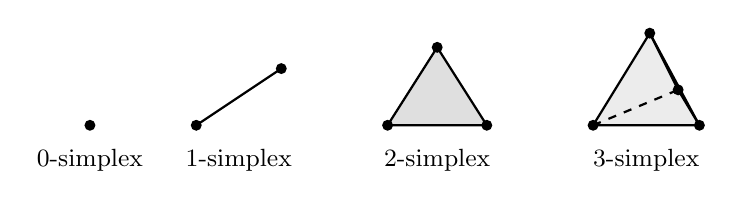
\begin{tikzpicture}[scale=0.9, v/.style={circle, fill=black, inner sep=1.4pt}]
  \node[v] at (0,0) {}; \node at (0,-0.5) {\small 0-simplex};
  \draw[thick] (1.5,0) node[v]{} -- (2.7,0.8) node[v]{}; \node at (2.1,-0.5) {\small 1-simplex};
  \fill[gray!25] (4.2,0) -- (5.6,0) -- (4.9,1.1) -- cycle;
  \draw[thick] (4.2,0) node[v]{} -- (5.6,0) node[v]{} -- (4.9,1.1) node[v]{} -- cycle; \node at (4.9,-0.5) {\small 2-simplex};
  \fill[gray!15] (7.1,0) -- (8.6,0) -- (7.9,1.3) -- cycle; \fill[gray!30] (8.6,0) -- (8.3,0.5) -- (7.9,1.3) -- cycle;
  \draw[thick] (7.1,0) node[v]{} -- (8.6,0) node[v]{} -- (7.9,1.3) node[v]{} -- cycle;
  \draw[thick] (8.6,0) -- (8.3,0.5) node[v]{} -- (7.9,1.3); \draw[thick, dashed] (7.1,0) -- (8.3,0.5);
  \node at (7.85,-0.5) {\small 3-simplex};
\end{tikzpicture}
\caption{Simplices of dimension 0 to 3.}\label{fig:simplices}
\end{figure}

\begin{definition}[Simplicial complex, {\cite{edelsbrunnerletscherzomorodian2002}}]
A \emph{simplicial complex} $K$ is a finite collection of simplices such that (i) every face of a simplex of $K$ is in $K$, and (ii) any two simplices of $K$ are disjoint or intersect in a common face.
Its \emph{vertex set} is the set of its 0-simplices.
\end{definition}

\begin{definition}[Abstract simplicial complex, {\cite{zomorodiancarlsson2005}}]
An \emph{abstract simplicial complex} on a vertex set $V$ is a collection $S$ of finite nonempty subsets of $V$ such that $\{v\} \in S$ for every $v \in V$, and $\tau \subseteq \sigma \in S$ implies $\tau \in S$.
A $k$-simplex is a set of $k+1$ vertices. Placing the vertices in general position gives a \emph{geometric realization} $|S|$.
\end{definition}
The abstract version only records which vertices span simplices, and it is the form in which nerves and Mapper graphs show up later on.
We write $[v_0, \dots, v_n]$ for a geometric simplex and $\{v_0, \dots, v_n\}$ for an abstract one.

\begin{example}\label{ex:complex}
On the vertex set $V = \{a, b, c, d\}$, let
\[
  K = \big\{ \{a\}, \{b\}, \{c\}, \{d\}, \{a,b\}, \{a,c\}, \{b,c\}, \{c,d\}, \{a,b,c\} \big\}.
\]
Every nonempty subset of a set in $K$ is also in $K$, so $K$ is an abstract simplicial complex with four 0-simplices, four 1-simplices, and one 2-simplex.
Its realization $|K|$ is a filled triangle with an edge attached at $c$ (Figure~\ref{fig:complex}).
If we removed $\{a,b\}$, the collection would no longer be a simplicial complex, since $\{a,b\}$ is a subset of $\{a,b,c\}$.
\end{example}

\begin{figure}[htbp]
\centering
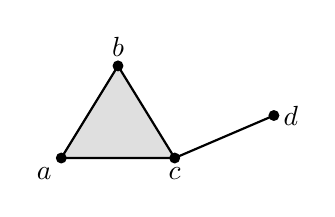
\begin{tikzpicture}[scale=0.9, v/.style={circle, fill=black, inner sep=1.4pt}]
  \fill[gray!25] (0,0) -- (1.6,0) -- (0.8,1.3) -- cycle;
  \draw[thick] (0,0) node[v]{} -- (1.6,0) node[v]{} -- (0.8,1.3) node[v]{} -- cycle;
  \draw[thick] (1.6,0) -- (3.0,0.6) node[v]{};
  \node[below left] at (0,0) {$a$}; \node[below] at (1.6,0) {$c$}; \node[above] at (0.8,1.3) {$b$}; \node[right] at (3.0,0.6) {$d$};
\end{tikzpicture}
\caption{The realization $|K|$ of the complex in Example~\ref{ex:complex}.}\label{fig:complex}
\end{figure}

\subsection{Skeleta and Graphs}
\begin{definition}[Skeleton, {\cite{edelsbrunnerharerpatel2008}}]
The \emph{$k$-skeleton} $K^{(k)}$ of a simplicial complex $K$ is the subcomplex of all simplices of dimension at most $k$. The 0-skeleton is the vertex set.
\end{definition}
By the abstract definition, a finite simple graph $G = (V, E)$, one with no edge from a vertex to itself and no repeated edges, is a simplicial complex of dimension at most one, with its vertices as 0-simplices and its edges as 1-simplices.
Its realization $|G|$, the graph viewed as a topological space, is a \emph{topological graph}.

\begin{example}\label{ex:graph}
Let $K$ be the complex of Example~\ref{ex:complex}. Its 1-skeleton is the graph $G = K^{(1)}$ with vertices $\{a,b,c,d\}$ and edges $\{a,b\}, \{a,c\}, \{b,c\}, \{c,d\}$.
The graph $G$ has one cycle, $a \to b \to c \to a$, and in $K$ the triangle fills it.
A graph can therefore show a loop that the complex it came from does not have, which is exactly what happens in Section~\ref{sec:loops}.
\end{example}

\subsection{Nerves}
\begin{definition}[Nerve, {\cite{singh2007mapper,hatcher2001}}]
Let $\mathcal U = \{U_\alpha\}_{\alpha \in A}$ be a finite cover of a space $X$ by nonempty sets.
The \emph{nerve} $N(\mathcal U)$ is the abstract simplicial complex with vertex set $A$ in which a set $\{\alpha_0, \dots, \alpha_k\} \subseteq A$ spans a $k$-simplex if and only if $U_{\alpha_0} \cap \cdots \cap U_{\alpha_k} \neq \emptyset$.
\end{definition}

\begin{example}\label{ex:nerve}
Cover a circle by three arcs, each overlapping the next, with no point in all three.
The nerve has three vertices and three edges but no triangle, so it is a hollow triangle, homotopy equivalent to the circle.
Cover a disk instead by three disks that share a common point. The nerve is then a filled triangle, homotopy equivalent to a point, and so to the disk (Figure~\ref{fig:nerve}).
\end{example}

\begin{figure}[htbp]
\centering
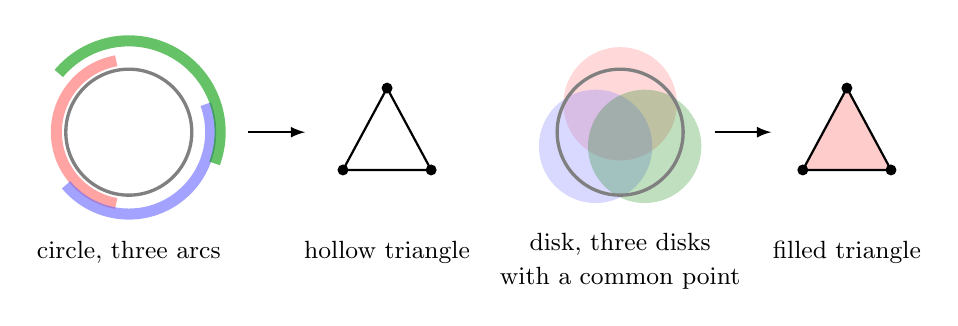
\begin{tikzpicture}[scale=0.8, v/.style={circle, fill=black, inner sep=1.4pt}]
  \draw[very thick, gray] (0,0) circle (1);
  \draw[line width=4pt, red!60, opacity=0.6] (100:1.15) arc (100:260:1.15);
  \draw[line width=4pt, blue!60, opacity=0.6] (220:1.3) arc (220:380:1.3);
  \draw[line width=4pt, green!60!black, opacity=0.6] (340:1.45) arc (340:500:1.45);
  \node at (0,-1.9) {\small circle, three arcs};
  \draw[-latex, thick] (1.9,0) -- (2.8,0);
  \draw[thick] (3.4,-0.6) node[v]{} -- (4.8,-0.6) node[v]{} -- (4.1,0.7) node[v]{} -- cycle;
  \node at (4.1,-1.9) {\small hollow triangle};
  \begin{scope}[xshift=7.8cm]
  % three disks of radius 0.9 centred 0.45 from the origin: together they cover the unit disk, and all contain the origin
  \fill[red!50, opacity=0.3] (90:0.45) circle (0.9); \fill[blue!50, opacity=0.3] (210:0.45) circle (0.9); \fill[green!50!black, opacity=0.25] (330:0.45) circle (0.9);
  \draw[very thick, gray] (0,0) circle (1);
  \node[align=center] at (0,-2.05) {\small disk, three disks\\\small with a common point};
  \draw[-latex, thick] (1.5,0) -- (2.4,0);
  \fill[red!20] (2.9,-0.6) -- (4.3,-0.6) -- (3.6,0.7) -- cycle;
  \draw[thick] (2.9,-0.6) node[v]{} -- (4.3,-0.6) node[v]{} -- (3.6,0.7) node[v]{} -- cycle;
  \node at (3.6,-1.9) {\small filled triangle};
  \end{scope}
\end{tikzpicture}
\caption{Two covers and their nerves (Example~\ref{ex:nerve}).}\label{fig:nerve}
\end{figure}

\subsection{The Nerve Theorem}
In both of these examples, the nerve has the shape of the space, and the nerve theorem tells us when this holds.

\begin{theorem}[Nerve theorem, {\cite[Cor.~4G.3]{hatcher2001}}]\label{thm:nerve}
If $X \subseteq \R^n$ and $\mathcal U$ is an open cover of $X$ in which every nonempty finite intersection of sets is contractible, then $X \simeq |N(\mathcal U)|$.
\end{theorem}
Hatcher states the theorem for paracompact spaces, a class that includes every metric space and so every subset of $\R^n$ \parencite[Thm.~41.4]{munkres2000topology}.
The idea is that each simplex of the nerve stands for a contractible piece of $X$, so passing to the nerve neither adds nor removes components or loops.

As we will see in Section~\ref{sec:mapper}, Mapper is the nerve of a cover built from the space, so if every nonempty intersection in that cover were contractible, the nerve theorem would make Mapper homotopy equivalent to the space itself.

\begin{remark}
Covers built from data are rarely this well behaved. A cluster of data points is a finite set, and a finite set with more than one point is never contractible, so the nerve theorem cannot apply to a sample literally. We instead read Mapper on a sample as a stand-in for the nerve of a cover of the unobserved space the sample comes from, and the intersections in that cover need not be contractible either. Therefore, a Mapper graph need not have the shape of the underlying space, and this is why Sections~\ref{sec:certify} and~\ref{sec:shape} test its features before we trust them.
\end{remark}

\subsection{Homology and Betti Numbers}\label{sec:homology}
\begin{definition}[Simplicial homology, {\cite{hatcher2001}}]
Let $K$ be an abstract simplicial complex. For each $k \ge 0$, let $C_k$ be the $\Z_2$-vector space with basis the $k$-simplices of $K$.
For $k \ge 1$, the \emph{boundary map} $\partial_k : C_k \to C_{k-1}$ is the linear map with
\[
  \partial_k \sigma = \sum_{v \in \sigma} \sigma \setminus \{v\}
\]
on each $k$-simplex $\sigma$, and $\partial_0 : C_0 \to 0$ is the zero map.
Since $\partial_k \circ \partial_{k+1} = 0$ \parencite[Lemma~2.1]{hatcher2001}, $\operatorname{im} \partial_{k+1} \subseteq \ker \partial_k$, and the $k$-th \emph{homology group} is the quotient
\[
  H_k(K) = \ker \partial_k / \operatorname{im} \partial_{k+1}.
\]
In particular, $H_0(K) = C_0 / \operatorname{im} \partial_1$.
Elements of $\ker \partial_k$ are \emph{$k$-cycles} and elements of $\operatorname{im} \partial_{k+1}$ are \emph{$k$-boundaries}.
The $k$-th \emph{Betti number} is $b_k(K) = \dim H_k(K) = \dim \ker \partial_k - \rank \partial_{k+1}$.
\end{definition}
So $b_1$ counts the independent loops that 2-simplices do not fill in, and $b_0$ counts connected components \parencite[Prop.~2.7]{hatcher2001}.
For a general space $X$, $H_k(X)$ is singular homology, which agrees with simplicial homology when $X$ is a simplicial complex \parencite[Thm.~2.27 and p.~153]{hatcher2001}, so we write $b_k(X)$ for both.

\begin{example}\label{ex:homology}
Take the complex $K$ of Example~\ref{ex:complex} (Figure~\ref{fig:complex}) and its 1-skeleton $G = K^{(1)}$.
The three triangle edges form a 1-cycle $z = \{a,b\} + \{b,c\} + \{a,c\}$, since $\partial_1 z = (a+b) + (b+c) + (a+c) = 0$ over $\Z_2$.
Any sum of edges that includes $\{c,d\}$ has $d$ in its boundary, so $\ker \partial_1$ is spanned by $z$ alone.
The graph $G$ keeps the three edges around $a$, $b$, $c$ but not the 2-simplex $\{a,b,c\}$, so $\operatorname{im} \partial_2 = 0$, the class of $z$ spans $H_1(G)$, and $b_1(G) = 1$.
In $K$, $\partial_2 \{a,b,c\} = z$, so $z$ is a boundary, $H_1(K) = 0$, and $b_1(K) = 0$.
\end{example}

For a finite graph $G$ with $V$ vertices, $E$ edges, and $C$ connected components, the Euler characteristic gives $V - E = b_0 - b_1$ with $b_0 = C$, so
\begin{equation}\label{eq:graph-b1}
  b_1(G) = E - V + C.
\end{equation}
The number $b_1(G)$ is the cycle rank of $G$, its number of independent cycles. Following topology, we call these loops, not to be confused with a loop in the graph-theoretic sense, an edge from a vertex to itself; Mapper graphs have no such edges.
In a complex of dimension two, 2-simplices can fill loops, and by rank--nullity
\begin{equation}\label{eq:complex-b1}
  b_1(K) = E - V + C - \rank \partial_2.
\end{equation}
Equation~\eqref{eq:complex-b1} is how Section~\ref{sec:loops} computes the loops of the full nerve.

%======================================================================
\section{The Mapper Algorithm}\label{sec:mapper}
%======================================================================
Singh, M\'emoli, and Carlsson introduced Mapper in 2007 \parencite{singh2007mapper}.
We first describe the topological version, which works on a space, and then the statistical version, which works on a finite sample and is the version that we run on pitch data.

\subsection{Topological Mapper}
\begin{definition}[Mapper, {\cite{singh2007mapper,deymemoliwang2017}}]
Let $f : X \to Z$ be continuous and let $\mathcal U = \{U_\alpha\}$ be a finite open cover of $Z$.
Split each preimage $f^{-1}(U_\alpha)$ into its path components. Together they form the \emph{pullback cover} $f^*\mathcal U$ of $X$.
The \emph{Mapper} is its nerve, $M(\mathcal U, f) = N(f^*\mathcal U)$.
\end{definition}
Dey, M\'emoli, and Wang showed that the loops of a Mapper are controlled by those of $X$.

\begin{theorem}[Dey--M\'emoli--Wang, {\cite[Thm.~8]{deymemoliwang2017}}]\label{thm:dmw}
If $\mathcal U$ is a finite open cover of a compact, path-connected space $X$ by path-connected sets, the nerve map $\varphi : X \to |N(\mathcal U)|$ induces a surjection $H_1(X) \to H_1(|N(\mathcal U)|)$, with $\Z_2$ coefficients.
\end{theorem}
Here $\varphi(x) = \sum_\alpha \rho_\alpha(x)\, u_\alpha$, where $u_\alpha$ is the vertex of $U_\alpha$ and $\{\rho_\alpha\}$ are continuous functions $X \to [0,1]$ with $\rho_\alpha$ supported in $U_\alpha$ and $\sum_\alpha \rho_\alpha = 1$, so each point goes to a weighted average of the vertices of the sets that contain it \parencite[Sec.~3.1]{deymemoliwang2017}. If $X$ is not path-connected, each set of the cover lies in one path component, so the theorem applies to each component separately.
When $X$ is compact and each preimage $f^{-1}(U_\alpha)$ has finitely many path components and they are open, the pullback cover is such a cover \parencite[Def.~14]{deymemoliwang2017}, and therefore \parencite[Thm.~18]{deymemoliwang2017}
\begin{equation}\label{eq:mapper-b1}
  b_1(M(\mathcal U, f)) \le b_1(X).
\end{equation}
This bound concerns the nerve, which is a simplicial complex. However, Mapper software such as KeplerMapper outputs only its 1-skeleton, whose loops are not bounded this way (Example~\ref{ex:homology}), and Section~\ref{sec:loops} shows the difference in our data.

\subsection{Statistical Mapper}
A \emph{point cloud} is a finite set $P \subseteq \R^n$ with Euclidean distance.
In the statistical version of Mapper, clustering plays the role of path components, and each preimage $f^{-1}(U_\alpha) \subseteq P$ is split into clusters \parencite{singh2007mapper}.
The algorithm has four steps:
\begin{enumerate}
  \item choose a \emph{lens} $f : P \to \R^k$;
  \item cover $f(P)$ by overlapping open sets $\mathcal U = \{U_\alpha\}$;
  \item cluster each preimage, in the full space $\R^n$;
  \item form the \emph{Mapper graph}, with one vertex per cluster and one edge for each pair of clusters that share a point.
\end{enumerate}
Steps 1--3 build a cover of $P$, apart from noise points, and step 4 takes its nerve \parencite{singh2007mapper}, keeping only the 1-skeleton.
The lens decides which points get clustered at the same time, since only points in the same preimage are clustered together, while the clustering itself uses all $n$ coordinates.

\begin{example}\label{ex:toy}
We follow one example through the rest of this section and the next.
Take the 240 noisy points $P$ on a circle of radius 1 shown in Figure~\ref{fig:toy}.
Its lens will be one-dimensional and its cover a set of intervals, whereas our real analysis uses a two-dimensional lens and squares, but each step works the same way.
The four parts below build Mapper on this circle, one step each.
\end{example}

\subsubsection{The Lens: Principal Component Analysis}
Principal component analysis (PCA) goes back to \textcite{pearson1901}, and it finds new uncorrelated variables, linear combinations of the old ones, that successively capture as much variance as possible \parencite{jolliffecadima2016}.
Among the Mapper applications reviewed by \textcite{madukpe2026review}, PCA is the most commonly used lens, and we use a two-dimensional PCA lens as well.

Let the data be $m$ observations of $n$ variables, and subtract each column's mean to obtain the centered matrix $\mathbf A \in \R^{m \times n}$.
We center the data because variance is measured around the mean, and after centering the covariance matrix is simply $S = \frac{1}{m-1}\mathbf A^{\mathsf T}\mathbf A$ \parencite{jolliffecadima2016}.
Its diagonal entries are the variances of the variables and its off-diagonal entries the covariances, and the variance of the data along a unit vector $v$ is $v^{\mathsf T} S v$.

\begin{theorem}[Singular value decomposition, {\cite{axler2024ladr}}]
Let $\mathbf A$ have rank $r \ge 1$. Then $\mathbf A = \mathbf U \boldsymbol\Sigma \mathbf V^{\mathsf T}$, where $\mathbf U \in \R^{m \times r}$ and $\mathbf V \in \R^{n \times r}$ have orthonormal columns and $\boldsymbol\Sigma = \operatorname{diag}(\sigma_1 \ge \cdots \ge \sigma_r > 0)$.
\end{theorem}
The columns $v_i$ of $\mathbf V$ are eigenvectors of $\mathbf A^{\mathsf T}\mathbf A$ with eigenvalues $\sigma_i^2$, and they are the \emph{principal directions}: $v_1$ maximizes $v^{\mathsf T} S v$ over unit vectors, each later $v_i$ does the same among unit vectors orthogonal to the earlier ones, and the variance along $v_i$ is $\lambda_i = \sigma_i^2/(m-1)$ \parencite{jolliffecadima2016}.
Keeping the first $k$ directions, $\mathbf V_k = [v_1 \cdots v_k]$, the lens is $f(x) = \mathbf V_k^{\mathsf T} (x - \bar x)$, where $\bar x$ is the mean, and component $j$ explains the proportion $\lambda_j / \sum_l \lambda_l$ of the variance.

For this paper, we take $k = 2$.
Since the cover lives in $\R^k$, with ten intervals per axis, $k = 2$ gives 100 cubes while $k = 3$ would give 1{,}000 cubes for the same \NShapes{} shapes, and a two-dimensional lens also has the advantage of being something that we can actually draw and read.
Because PCA is linear, it can flatten curved structure, but we accept this since clustering happens in the full space, and Section~\ref{sec:certify} repeats the stability analysis with three other lenses, including the nonlinear Isomap \parencite{tenenbaum2000isomap}.

For the circle of Example~\ref{ex:toy}, the variance is nearly the same in every direction, so the first principal direction is not well determined, and we choose the vertical direction, which gives the height $f(x,y) = y$ as the lens.

\begin{figure}[htbp]
\centering
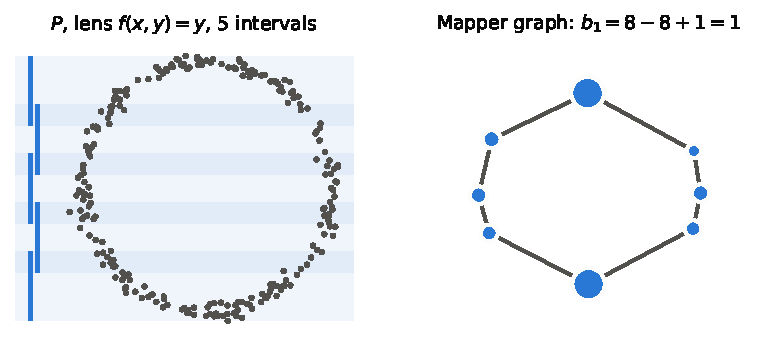
\includegraphics[width=0.75\textwidth]{toy_mapper.pdf}
\caption{Mapper on a noisy circle (Example~\ref{ex:toy}). Left, the 240 points and the five intervals of the cover. Right, the resulting graph.}\label{fig:toy}
\end{figure}

\subsubsection{The Cover}
The image $f(P) \subseteq \R^k$ is covered by overlapping hypercubes, where each axis is cut into intervals of equal length, and neighboring intervals share a fixed percentage of their length \parencite{singh2007mapper,madukpe2026review}.
Each hypercube is a product $I_1 \times \cdots \times I_k$ of one interval from each axis, so ten intervals per axis give $10^k$ sets $U_\alpha$, and since $P$ is finite we may take them open without changing which points each one contains.
Two parameters set the resolution, the number of intervals and the percentage overlap \parencite{singh2007mapper}. The resulting graph depends on both, and tuning them on real data is not easy \parencite{carrieremicheloudot2018}.
We use ten intervals per axis with 30\% overlap and test the results over a grid of alternatives (Section~\ref{sec:certify}).
For the circle, we cover the range of heights by five intervals with 30\% overlap, and since the overlap is less than 50\%, an interval does not reach past its neighbor, so no height lies in three intervals at once.

\subsubsection{Clustering: DBSCAN}\label{sec:dbscan}
DBSCAN was introduced by \textcite{ester1996dbscan} in 1996, and it is the second most common choice in reviewed Mapper applications after hierarchical clustering \parencite{madukpe2026review}.
It needs no preset number of clusters, finds clusters of arbitrary shape, and labels isolated points as noise.
DBSCAN runs separately on each preimage in step 3, so fix one such point cloud $P$ with distance $d$, a radius $\varepsilon > 0$, and a count $M \in \N$ (called Eps and MinPts by \textcite{ester1996dbscan}).

\begin{definition}[Density reachability, {\cite[Defs.~1--4]{ester1996dbscan}}]
The \emph{$\varepsilon$-neighborhood} of $p \in P$ is $N_\varepsilon(p) = \{ q \in P : d(p,q) \le \varepsilon \}$, and $p$ is a \emph{core point} if $N_\varepsilon(p)$ contains at least $M$ points.
A point $p$ is \emph{directly density-reachable} from $q$ if $p \in N_\varepsilon(q)$ and $q$ is a core point, and \emph{density-reachable} from $q$ if there is a chain $q = p_1, p_2, \dots, p_\ell = p$, with $\ell \ge 2$, in which each $p_{i+1}$ is directly density-reachable from $p_i$.
Points $p$ and $q$ are \emph{density-connected} if both are density-reachable from some common point $o$.
\end{definition}
\begin{definition}[Cluster and noise, {\cite[Defs.~5--6]{ester1996dbscan}}]
A \emph{cluster} is a nonempty $C \subseteq P$ such that (i) if $p \in C$ and $q$ is density-reachable from $p$, then $q \in C$ (maximality), and (ii) any two points of $C$ are density-connected (connectivity), and (iii) $C$ contains a core point.
Points of a cluster that are not core points are \emph{border points}.
\emph{Noise} is the set of points of $P$ in no cluster, so it depends on the chosen $(\varepsilon, M)$.
\end{definition}
We require $\ell \ge 2$ and condition (iii). If $\ell = 1$ were allowed, every point would be density-reachable from itself, a lone non-core point would form a cluster of its own, and there would be no noise. Even with $\ell \ge 2$, a lone border point $b$ near a core point $c$ would satisfy (i) and (ii), since nothing is density-reachable from $b$ and $b$ is density-connected to itself through $c$. \textcite[p.~228]{ester1996dbscan} note that every cluster contains a core point, and (iii) makes that explicit.
\begin{lemma}[{\cite[Lemma~2]{ester1996dbscan}}]
If $C$ is a cluster and $p \in C$ is a core point, then $C = \{ o \in P : o \text{ is density-reachable from } p \}$.
\end{lemma}
The algorithm loops over the points and expands a new cluster from each unclassified core point \parencite[p.~229]{ester1996dbscan}. A point that isn't a core point gets marked as noise for now, and a border point first marked as noise is relabeled if a later cluster reaches it.
The lemma is why this works, since a cluster is determined by any one of its core points, so starting from an unclassified core point and collecting everything density-reachable from it recovers exactly its cluster.
Even though \textcite{ester1996dbscan} allow separate parameters for each cluster, their algorithm uses a single pair, and so do we, with $\varepsilon = 1.0$ in standardized units and $M = 4$.
Figure~\ref{fig:dbscan} illustrates the three kinds of point on a separate small example.

For the circle we use $\varepsilon = 0.25$ and $M = 3$.
DBSCAN then splits the five preimages into $1, 2, 2, 2, 1$ arcs, since the top and bottom intervals each meet the circle in one arc and the middle three meet it in two.

\begin{figure}[htbp]
\centering
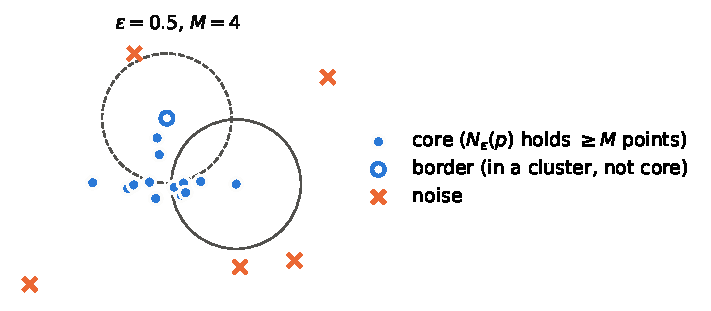
\includegraphics[width=0.6\textwidth]{dbscan_toy.pdf}
\caption{A separate illustration of core, border, and noise points, for $\varepsilon = 0.5$ and $M = 4$. Solid circle, a core point's $\varepsilon$-ball, which holds six points. Dashed circle, a border point's ball, which holds three points including a core point, so the border point joins the cluster. Crosses, noise points, each more than $\varepsilon$ from every core point.}\label{fig:dbscan}
\end{figure}

\subsubsection{The Mapper Graph}
Each cluster becomes a vertex, which we also call a node, and two clusters are joined by an edge when they share at least one point, which happens due to the overlap between neighboring cubes \parencite{singh2007mapper}.
The clusters form a cover of the non-noise part of $P$, and the graph is the 1-skeleton of its nerve, so while three clusters with a common point span a triangle in the nerve, the graph only keeps the three edges.
We run all four steps with KeplerMapper, a Python implementation that works with scikit-learn-compatible clustering and scaling algorithms \parencite{vanveen2019keplermapper,pedregosa2011sklearn}, developed under the scikit-tda project \parencite{keplermapper_repo}.

For the circle, no point lies in three intervals, so no three clusters share a point.
The graph has 8 vertices and 8 edges in one component, so by~\eqref{eq:graph-b1} it has $b_1 = 8 - 8 + 1 = 1$, and since there are no triangles, the nerve is the graph.
Mapper has recovered the single loop of the circle.

%======================================================================
\section{Data Collection and Processing}\label{sec:data}
%======================================================================
Major League Baseball's Statcast tracks every pitch in every game, and its data is publicly available to download and use \parencite{savantcsvdocs}.
Using the pybaseball package \parencite{ledoux_pybaseball}, we downloaded the data from Baseball Savant and preprocessed it into a set of pitch shapes, which we define below.
For the full details of the data and the code, see Appendix~\ref{app:repro}.

The main analysis uses every pitch from March 28 to November 4, 2025, which holds the regular season from that date on and the full postseason, bringing the total to \NPitches{} pitches.
This time frame gives us a full season of data, though it misses the first games of the season, the Tokyo Series on March 18 and 19 and the domestic openers on March 27, which account for under 1\% of the season's pitches.
We describe each pitch by eight of the measurements from Section~\ref{sec:statcast}, those being release speed, $\mathit{pfx}_x$, $\mathit{pfx}_z$, spin rate, spin axis, extension, and the horizontal and vertical release position, and we drop pitches that are missing any of them or a pitch type.

To handle handedness, left-handed pitchers are mirrored into the right-handed frame, so $\mathit{pfx}_x$ and the horizontal release position change sign and the spin axis $\theta$ becomes $360^\circ - \theta$.
Dealing with spin axis, we know it is an angle, so $359^\circ$ and $1^\circ$ point in almost the same direction even though they are far apart as numbers. We therefore encode it as the point $(\cos\theta, \sin\theta)$ on the unit circle, which gives nine coordinates in all.

An important definition is that of a \emph{pitch shape}, which, in our case, is the average of one pitcher's pitches of one Statcast label.
Averaging reduces pitch-to-pitch variation while keeping what is consistent about how a pitcher throws that pitch, and gives us \NShapes{} shapes in $\R^{\NFeatures}$, which we standardize to mean zero and unit variance.
We did not set a minimum pitch count for the fit. The median shape averages \MedianPitches{} pitches, but \PctLtFive\% average fewer than five and \PctLtTwenty\% fewer than twenty, and the \NSlow{} slow shapes (below 70 mph) have a median of \SlowMedian{} pitches and a quarter at \SlowQ{} or fewer.
The reason for not setting a minimum is that we want to see the full range of shapes, and Appendix~\ref{app:thin} repeats the main Mapper fit with minimum counts of 10 and 20.

For some of our analysis, we use a smaller set of coordinates that we call \emph{flight space}: velocity relative to the pitcher's fastest pitch shape, $\mathit{pfx}_x$, $\mathit{pfx}_z$, spin rate, and the spin axis, for six coordinates in all.
The reason for leaving out the delivery (release position and extension) and absolute velocity is that they make a pitcher's own pitches look alike, so the shapes would group by pitcher rather than by how the ball moves.

There are two other data sets that appear later in the paper, which use the same procedure, but from different time periods. The Stuff+ models of Section~\ref{sec:consequences} are trained on a separate pull from April 7, 2022 to July 31, 2024 (\StuffTrainN{} pitches), and the 2026 regular season and postseason through October 26 (\NPitchesTwentySix{} pitches) are used to replicate the flight-space check in Section~\ref{sec:shape} and the label-sensitivity result in Section~\ref{sec:consequences}.
Repeating these two on 2026 allows us to check whether they are specific to one season.

In general, each result uses the space that fits its question. The Mapper graph and its tests use pitch shapes in all nine coordinates, since the question is about the shape of what pitchers throw. The dense regions use single pitches in three coordinates (Section~\ref{sec:peaks}), since averaging would hide where individual pitches pile up. Flight space checks which results come from the flight of the ball rather than the delivery, and it is where we find a pitch's neighbors in Section~\ref{sec:consequences}, so that a pitcher's own delivery does not decide which shapes count as close.

%======================================================================
\section{Testing the Mapper Picture}\label{sec:certify}
%======================================================================
The graph that the Mapper algorithm produces gives us a solid picture of the data, but the graph depends on choices we make (the lens, the cover, and the clustering). It can also show structure that comes only from the covariance of the data, so we cannot simply read the graph and conclude that its features are real.
When we say a \emph{feature} we mean a property of the graph's shape, such as its number of components or the order of velocities along it, not an input variable in the machine-learning sense.

In order to test the features, we need to ask two simple questions. First, does a feature survive reasonable changes to the construction? Second, does a null model that lacks the structure produce it anyway?
After we answer these key questions, we compute the homology of the full nerve and two checks that do not use Mapper at all, those being persistent homology and density peaks.

We are not the first to have this worry.
\textcite{topaz2026null} shows that the covariance of data alone can make Mapper's groups of nodes look different, and proposes a Gaussian null with the sample covariance, which we arrived at independently.
As Topaz notes, failing to beat such a null does not prove that structure is absent, and the same holds for our results: when a feature does not beat the nulls, we conclude only that covariance alone can explain it.
To us, this is a cautionary tale, and we apply the null beyond groups of nodes to the graph's features, its loops, the homology of the point cloud, and its density peaks, in the spirit of hypothesis testing for persistent homology \parencite{robinsonturner2017,blumberg2014}.

\subsection{Stability}
A feature that appears for only one choice of parameters tells us more about the parameters than about the data.
For this reason, we refit the graph over a 27-point grid, with 8, 10, or 12 intervals per axis, 20, 30, or 40\% overlap, and $\varepsilon = 0.8$, 1.0, or 1.2.
In case it wasn't enough, we refit the graph 30 times on a random 80\% of pitchers, drawn without replacement, to see whether a feature depends on a handful of pitchers.
The lens is a choice as well, so every fit is repeated with four lenses, those being the PCA lens, velocity against induced vertical break, a two-dimensional Isomap embedding, and a one-dimensional density lens given by the mean distance to the ten nearest neighbors.

The nodes of one fit do not carry over to another fit, so we cannot follow a feature by tracking its nodes. Instead, we define each feature by the pitch shapes that the nodes contain.
Let $G$ be the Mapper graph of a fit and $G_0$ its largest connected component, measured by number of nodes. We can use the following terms to describe the features of $G$ relative to $G_0$.

We call shapes slower than 70 mph \emph{slow shapes}, which typically will be the eephus pitches and/or position players pitching (Section~\ref{sec:shape}).

\begin{definition}[Tracked features]\label{def:features}
\leavevmode
\begin{enumerate}[label=(\roman*), leftmargin=*]
  \item \emph{Component structure} is the number of connected components of $G$, together with the share of nodes that lie in $G_0$.
  \item \emph{Slow-pitch isolation} asks whether at least half of the slow shapes that land in some node lie only in nodes outside $G_0$. It is undefined in fits where every slow shape is noise.
  \item The \emph{velocity ordering} of two pitch types $\tau$ and $\tau'$ is defined as follows. Let $v_0$ be the node of $G_0$ with the highest share of type $\tau$ and $v_L$ the node of $G_0$ with the highest share of type $\tau'$, among nodes of at least 10 shapes. We take a shortest path $v_0, v_1, \dots, v_L$ in $G_0$ and compute Spearman's $\rho$ between the position $i$ and the mean velocity of the shapes in $v_i$. The ordering is present when $\rho \ge 0.7$, and it is undefined when the path has fewer than three nodes.
\end{enumerate}
\end{definition}
In our case, $\tau$ and $\tau'$ are the curveball and the four-seam fastball, the slowest and fastest of the common pitch types, so that the path spans the full range of velocities.

\subsection{Null Models}\label{sec:nulls}
A null model is a data set built to keep some of the structure of ours and throw away the rest.
If a null produces a feature as often as the real data does, then the feature comes from the structure the null keeps and not from anything more.
We use three nulls, and each is refit through the identical pipeline.

The \emph{Gaussian null} has the same mean and covariance as the shapes and no structure beyond these second moments. It is our main comparison, and we use it in every test.

The \emph{within-type shuffle} permutes each coordinate independently among shapes of the same pitch type, which keeps each type's marginal distributions but destroys the joint structure inside it. We use it alongside the Gaussian for the stability features and for loops.

The \emph{spin-pair shuffle} does the same but permutes $(\cos\theta, \sin\theta)$ together, so every shuffled shape still has a spin axis that could actually occur. In flight space, where spin is a larger share of the coordinates, it takes the place of the within-type shuffle.

A feature counts as evidence of structure only if the real data show more of it than the whole range that the nulls produce, for every null we compare against.
We draw 10 replicates of each null for every lens in the stability check, 5 for the nerve and for persistent homology, and 50 for the density peaks.

\subsection{Loops of the Full Nerve}\label{sec:nerveloops}
As we saw in Example~\ref{ex:homology}, a graph can have a loop that the full complex fills in, and we know that a Mapper graph is only the 1-skeleton of its nerve.
Throughout, a loop means what $b_1$ counts: for a graph, an independent cycle (Section~\ref{sec:homology}), and for the nerve, an independent cycle that its 2-simplices do not fill.
In order to see which loops actually survive, we compute the first Betti number of both the graph and the full nerve for every fit, those being the real fits as well as the null fits.
For the graph, this comes straight from~\eqref{eq:graph-b1}.
For the nerve, we add a 2-simplex for every three clusters with a common point and compute $\rank \partial_2$ over $\Z_2$, which gives us its $b_1$ by~\eqref{eq:complex-b1}.
We do not need to go any higher than 2-simplices, since simplices of dimension three and up cannot change $b_1$, so this is the $b_1$ of the full nerve.

It would be nice if Theorem~\ref{thm:dmw} told us how many nerve loops to expect, but unfortunately it does not apply directly, since our cover is made of DBSCAN clusters of a finite sample rather than path-connected open sets. So instead of leaning on the theorem, we lean on the null models (Section~\ref{sec:loops}).

\subsection{Persistent Homology}
Everything so far depends on Mapper, so independently we want to see whether the data have loops or gaps without using Mapper at all.
\begin{definition}[Vietoris--Rips complex and persistence]\label{def:persistence}
For a finite metric space $(P, \delta)$ and scale $t \in \R$, the \emph{Vietoris--Rips complex} is $\mathrm{Rips}_t(P) = \{ \emptyset \neq S \subseteq P : \diam S \le t \}$ \parencite{bauer2021ripser}.
As $t$ grows, these complexes are nested, and persistent homology records the scale $b$ at which each component or loop is born and the scale $d$ at which it dies \parencite{edelsbrunnerletscherzomorodian2002,zomorodiancarlsson2005}.
Its \emph{persistence} is $d - b$, and the \emph{persistence diagram} is the set of points $(b, d)$, one for each component or loop.
\end{definition}
In a persistence diagram, anything that dies soon after it is born sits near the diagonal $d = b$ and is usually read as noise, while points far from it are read as real structure \parencite{fasy2014confidence} (Figure~\ref{fig:rips}).
In general, an $H_0$ bar that lives a long time is a gap between groups of points, and a long $H_1$ bar is a loop.
We compute persistence over $\Z_2$ with Ripser \parencite{bauer2021ripser,tralie2018ripserpy}.
For $H_0$ we use all \NShapes{} standardized shapes. Computing $H_1$ is much more expensive, so for it we use five random subsamples of 1{,}000 shapes. We do the same for five Gaussian and five within-type-shuffle nulls.

We do not compute formal confidence sets. Instead, we compare with the nulls, measuring every persistence, real or null, as a multiple of one fixed length $u$, the median $H_0$ death of the real data, which is roughly the typical distance between neighboring shapes.
An $H_0$ bar is long-lived if it dies after $3u$, and an $H_1$ loop is persistent if its persistence exceeds $2u$. By the largest loop, we mean the largest loop persistence averaged over the five subsamples.
These cutoffs are our own convention relative to the pitch data, not a standard one.

\begin{figure}[htbp]
\centering
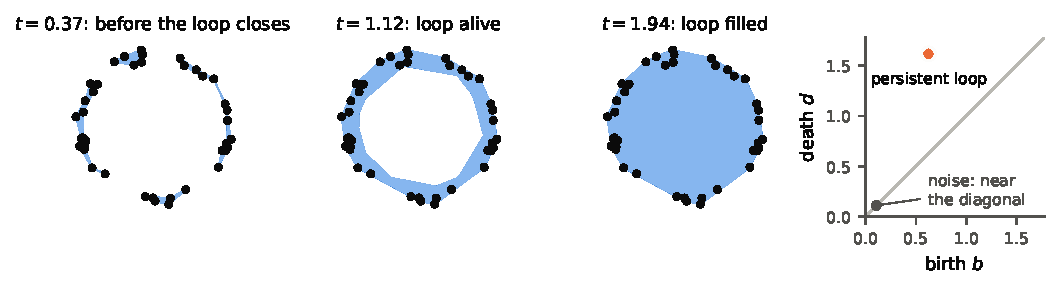
\includegraphics[width=\textwidth]{rips_toy.pdf}
\caption{A persistent loop on synthetic data (40 points from a noisy circle), not pitch data: Rips complexes at three scales and the $H_1$ persistence diagram. The loop has persistence \RipsPers, against \RipsNext{} for the next-longest loop.}\label{fig:rips}
\end{figure}

\FloatBarrier
\subsection{Density Peaks}\label{sec:peaks}
Vietoris--Rips persistence detects gaps, but it does not see density, so it cannot tell one dense region from several that are joined without a gap.
In order to look for dense regions, we follow \textcite{maloof2026classify} and compute the persistence of the superlevel sets of a smoothed density at the pitch level, meaning single pitches rather than pitch shapes.
Each peak of the density is born at its height and dies when it merges with a taller one, so a peak with high persistence is a dense region that stands out from its surroundings.
We divide each peak's persistence by the height of the tallest peak and call this its relative persistence.

As in their work, we describe each 2025 pitch by three numbers, those being its speed relative to the pitcher's 95th-percentile speed in that game, its horizontal break, and its induced vertical break ($\mathit{pfx}_x$ and $\mathit{pfx}_z$ in inches, left-handers mirrored).
We count the pitches on a $50^3$ grid and smooth the counts with a Gaussian of one grid cell (Appendix~\ref{app:repro}).

To test the peaks, we draw 50 Gaussian samples with the same mean, covariance, and number of pitches, run each through the same steps, and compare each real peak's relative persistence with the largest secondary peak of each sample, which gives us a Monte Carlo $p$-value.
The catch is that a Gaussian has only one peak, so this test only tells us that there is more than one.
For the small peaks, we lean on robustness instead, repeating the analysis with smoothing of 1.5 and 2 cells and on three random halves of the pitches, each against its own Gaussian null of 20 samples, and we say a peak appears in a variant if the variant has a peak within three grid cells of it.

%======================================================================
\section{The Shape of Pitch Space}\label{sec:shape}
%======================================================================
We now apply these methods to the 2025 pitch shapes. We first look at what the lens and the Mapper graph show, then test each of those observations, and finally ask what the results mean for how pitches are described.

\subsection{The PCA Lens}
The first two principal components explain \PCone\% and \PCtwo\% of the variance (Figure~\ref{fig:lens}).
The first separates fastballs from breaking balls, so the main pitch differentiator is the fastball-to-breaking-ball axis.
The second is mostly delivery (extension and release height) along with velocity, which describes the pitcher more than the pitch, with the slowest pitches living at the bottom.
Notice that offspeed pitches overlap fastballs in the lens because they typically move in the same direction, toward the arm side, and differ mainly in speed, spin, and vertical break ($\mathit{pfx}_z$).
From a hitter's point of view, an offspeed pitch is designed to appear like the pitcher's fastball, but either slower or with a different spin axis, to mess with the batter's timing.
Offspeed movement relative to the fastball is part of what lets a pitcher tunnel the two, making them appear the same to the batter longer, and leaving the batter less time to decide whether to swing or make good contact.
Our shapes describe a pitch's whole flight rather than its path at the tunneling point, which is about 24 feet from home plate \parencite{sayre2017tunnels}.
Clustering uses all nine coordinates, so this overlap in the lens does not force them into the same nodes.

\begin{figure}[htbp]
\centering
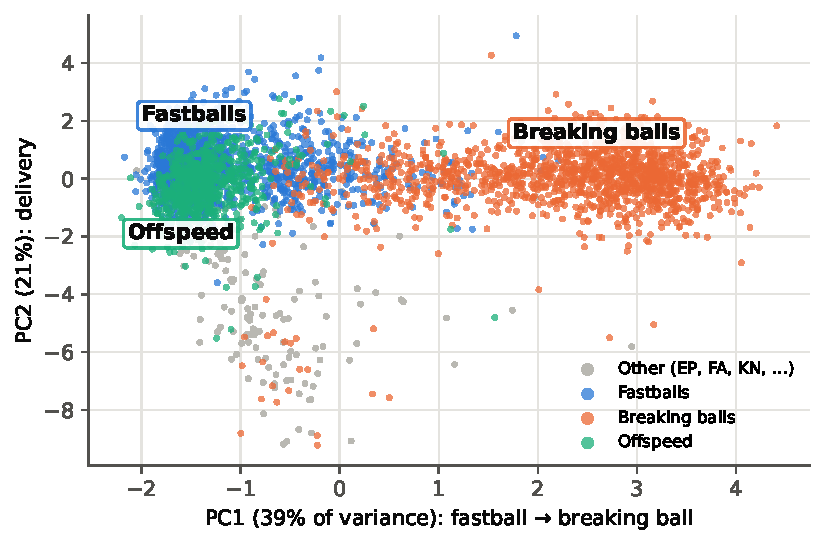
\includegraphics[width=0.7\textwidth]{lens_scatter.pdf}
\caption{The 2025 pitch shapes in the PCA lens, by pitch family.}\label{fig:lens}
\end{figure}

\FloatBarrier
\subsection{The Mapper Graph}
The Mapper graph (Figure~\ref{fig:graph}) has \NNodes{} nodes, \NEdges{} edges, and \NComponents{} components.
One large component holds \GiantShapes{} of the \NShapes{} shapes and runs from curveballs through sliders and cutters to fastballs and offspeed pitches, ordered by velocity.
Of the other components, \NSlowComps{} hold only the very slow pitches (eephus pitches and position players pitching), and the other \NOtherComps{} are single nodes holding a few ordinary sliders and cutters.
The remaining \NoiseShapes{} shapes fall in no node, since DBSCAN marks them as noise.
The graph also has many loops, and a band of sliders and cutters between the fastball and breaking-ball ends has the highest betweenness centrality.
Read at face value, the picture suggests a velocity ladder, a separate group of slow pitches, loops, and a slider--cutter band joining the families, and the next subsection tests each of these.

\begin{figure}[htbp]
\centering
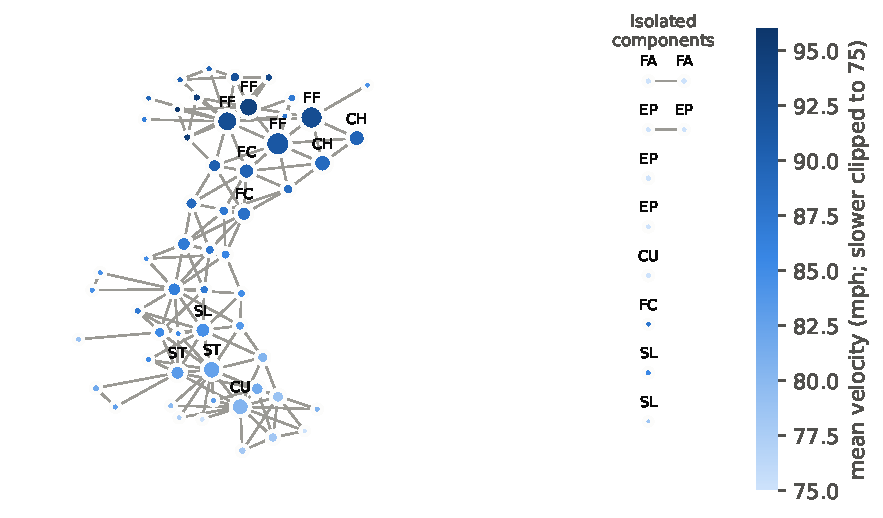
\includegraphics[width=0.75\textwidth]{mapper_graph.pdf}
\caption{The Mapper graph, nodes colored by mean velocity.}\label{fig:graph}
\end{figure}

\FloatBarrier
\subsection{What Survives Testing}\label{sec:tests}
\subsubsection{Velocity Ordering and Slow Pitches}
The velocity ordering and slow-pitch isolation of Definition~\ref{def:features} are stable across the parameter grid, the subsamples, and all four lenses, with the velocity ordering holding in \StabOrderMin\% of fits under every lens and slow-pitch isolation in \StabSlowLo--\StabSlowHi\%.
The results from the nulls reproduce the velocity ordering in \NullOrderMin\% of their fits, so this ladder from slow breaking balls up to hard fastballs comes from how velocity, movement, and spin vary together and not from hidden topology.
Slow-pitch isolation appears in only \NullSlowLo--\NullSlowHi\% of the null fits where it is defined, and most within-type shuffles leave it undefined, so it passes, but only weakly. The flight-space check below traces it to absolute velocity and delivery.
The slider--cutter band changed when we changed the lens, and the nulls reproduced it, so it is not structure beyond the continuum. It still remains a real description of where sliders and cutters sit, between the breaking-ball and fastball. 
Slider and cutter is also the most common boundary pair in Section~\ref{sec:consequences}, and \BandBoundaryPct\% of those boundary pitches sit in the band's nodes, against \BandAllPct\% of sliders and cutters in general. The band is what a continuum with this covariance looks like, not a bridge between separate groups.

\begin{figure}[t]
\centering
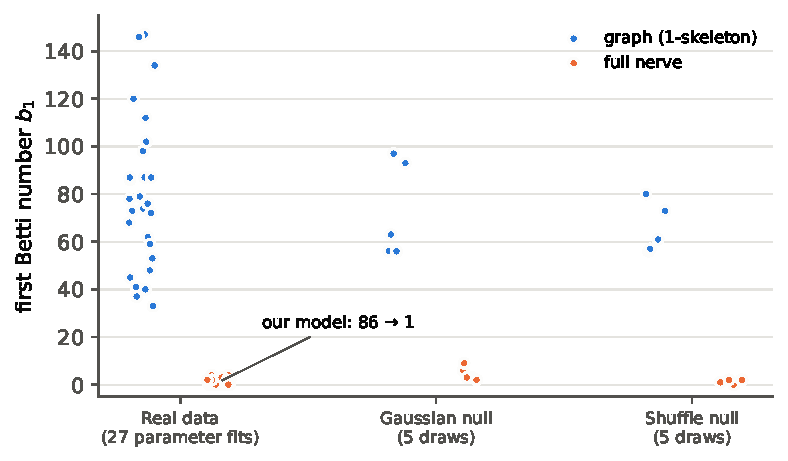
\includegraphics[width=0.6\textwidth]{nerve_b1.pdf}
\caption{First Betti number of the Mapper graph and of the full nerve, for real fits and null models.}\label{fig:nerveb1}
\end{figure}

\subsubsection{Loops and Gaps}\label{sec:loops}
By~\eqref{eq:graph-b1} the graph has $b_1 = \NEdges - \NNodes + \NComponents = \GraphBone$.
Its nerve adds a 2-simplex for every three clusters with a common point, and $\partial_2$ has rank \NerveRank{} over $\Z_2$, so by~\eqref{eq:complex-b1} the nerve has $b_1 = \GraphBone - \NerveRank = \NerveBone$.
Across the 27 parameter choices, the graph has \GridGraphBoneMin--\GridGraphBoneMax{} loops and the nerve \GridNerveBoneMin--\GridNerveBoneMax, and the nulls show the same pattern, with nerves of \NullNerveBoneMin--\NullNerveBoneMax{} loops (Figure~\ref{fig:nerveb1}).
The reason for this gap is that the graph's loops come from only reading its 1-skeleton, and the few nerve loops that are left are no more than what the nulls produce.
On the other hand, persistent homology, which does not use Mapper at all, also finds no persistent loop (Figure~\ref{fig:persistence}).
This agrees with Theorem~\ref{thm:dmw}, where a space with no loops has a nerve with no loops, although, as we saw in Section~\ref{sec:nerveloops}, the theorem does not strictly apply to our clusters, so the two together fall short of a result.
For baseball, this means we find no chain of pitch types that leads around and back to where it started, so a loop in a Mapper picture of pitch data should not be read as one without these checks.

\begin{figure}[!b]
\centering
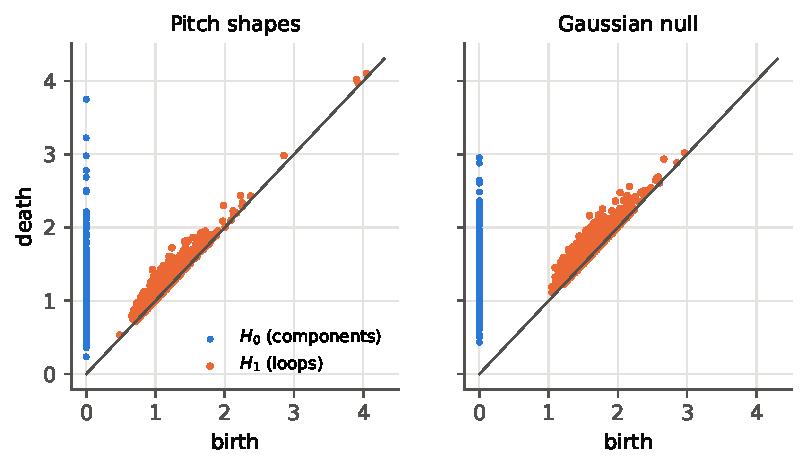
\includegraphics[width=0.55\textwidth]{persistence.pdf}
\caption{Persistence diagrams of one random subsample of 1{,}000 pitch shapes and of a same-covariance Gaussian, in multiples of $u$, the median $H_0$ death of the real data. Every loop lies well below the dashed line, where persistence is $2u$, and the few tall $H_0$ points are single unusual shapes, such as knuckleballs and slow curves.}\label{fig:persistence}
\end{figure}

The same persistence diagrams speak to gaps.
On all \NShapes{} shapes, the data have \PHRealLongBars{} long-lived $H_0$ bars against \PHGaussLongBarsLo--\PHGaussLongBarsHi{} for the Gaussian, so they have no more gaps than covariance alone produces, and the Gaussian's typical gaps between neighboring shapes are \PHGaussHzeroMedian{} times as large.
The long-lived bars split off \PHLongSingles{} single shapes and a few groups of at most \PHLongMaxGroup, mostly knuckleballs, eephus pitches, and slow curves, and none separates a group of ordinary pitches.
Put simply, nothing like an empty zone sits between, say, sliders and cutters.

\subsubsection{Dense Regions}
At the level of individual pitches, the density has three robust peaks, for fastballs, breaking balls, and offspeed pitches.
The breaking-ball and offspeed peaks have relative persistence \PeakBB{} and \PeakCH, each beats every null replicate ($p = \PeakP$, the smallest value 50 replicates allow), and both appear at every smoothing level and in every half of the data, close to where \textcite{maloof2026classify} find them for college pitches.
Two smaller bumps, one curveball-like (\PeakCurve) and one sweeper-like (\PeakSweep), do not hold up under every check, so we claim neither.
Individual pitches, then, pile up in three heaps, around fastballs, breaking balls, and offspeed pitches, and not around the finer pitch types that Statcast uses.

\subsubsection{Flight Space}
In flight space (Section~\ref{sec:data}), which keeps only the flight of the ball, most results hold in both 2025 and 2026 (Table~\ref{tab:flight}). The graph is connected, and there are fewer gaps than the nulls produce.
Two things change. The slow shapes are no longer isolated, so what sets them apart is absolute velocity and delivery rather than the flight of the ball.
There is one loose end. In both seasons, flight space shows a hint of a loop, as its persistence sits just over our cutoff and, at some parameter choices, the nerve keeps more loops than either null. 
Neither hint holds up, though. The persistence is no larger than what most within-type shuffles produce, and at other parameter choices the nerve has no loops at all. Ultimately, these data cannot tell this loop apart from chance.

\begin{table}[htbp]
\centering
\small
\begin{tabular}{lccc}
\toprule
 & Nine coordinates & \multicolumn{2}{c}{Flight space} \\
\cmidrule(lr){3-4}
 & 2025 & 2025 & 2026 \\
\midrule
Components (chosen parameters) & \NComponents & \FlComp & \FlSixComp \\
Slow-pitch isolation (\% of fits) & \StabSlowPCALo--\StabSlowPCAHi & \FlSlowIso & \FlSixSlowIso \\
Nerve $b_1$ (grid range) & \GridNerveBoneMin--\GridNerveBoneMax{} (\NullNerveBoneMin--\NullNerveBoneMax) & \FlGridNerveMin--\FlGridNerveMax{} (\FlNullNerveMin--\FlNullNerveMax) & \FlSixGridNerveMin--\FlSixGridNerveMax{} (\FlSixNullNerveMin--\FlSixNullNerveMax) \\
Long-lived $H_0$ bars & \PHRealLongBars{} (\PHGaussLongBarsLo--\PHGaussLongBarsHi) & \FlLongBars{} (\FlGaussLongBarsLo--\FlGaussLongBarsHi) & \FlSixLongBars{} (\FlSixGaussLo--\FlSixGaussHi) \\
Largest loop persistence & \PHMaxPers{} (\PHGaussMaxPersLo--\PHGaussMaxPersHi) & \FlMaxPers{} (\FlGaussMaxPersLo--\FlGaussMaxPersHi) & \FlSixMaxPers{} (\FlSixGaussMaxPersLo--\FlSixGaussMaxPersHi) \\
\bottomrule
\end{tabular}
\caption{Shape results in all nine coordinates and in flight space (PCA lens). Parentheses give the nulls: Gaussian and within-type shuffle for nerve $b_1$, and Gaussian for $H_0$ bars and loop persistence. Persistence is in multiples of $u$, the median $H_0$ death of the real data in that space, and a loop is persistent above $2u$.}\label{tab:flight}
\end{table}

\FloatBarrier
\subsection{What the Shape Tells Us}\label{sec:meaning}
Ultimately, each result that survives testing changes how pitch data should be read, and in our case, what the geometry says about the labels we put on pitches.
In a baseball context, the picture is simple.
A pitch type is a name for a region of one continuous space, and the regions run into each other, so a slider and a cutter, or a changeup and a splitter, can be nearly the same shape under two different names.
Only the three broad families stand out on their own, and only the slowest pitches sit apart.

This matters because the labeling is used from scouting reports to pitch grades, and the current system treats these labels as a natural grouping.
If the labels cut a continuum, then a pitch's grade, the pitches it is compared with, and even the ideas for how to improve it depend partly on where the line falls, and Section~\ref{sec:consequences} looks at what that means for evaluating and designing pitches.

%======================================================================
\section{Consequences for Pitch Evaluation and Design}\label{sec:consequences}
%======================================================================
One key inspiration for this work was the study of \textcite{lum2013extracting}, who built a topological network from NBA player statistics, using a construction with the same inputs as Mapper, and found 13 player positions in place of the traditional five.
Basketball has grown into a sport where the five positions cannot accurately describe the players' role on the court at any given time.
Take a player like Victor Wembanyama, a seven-footer who is a dominant shot-blocker and rebounder, but also a shot creator from anywhere on the court. He is not a traditional center, forward, or guard, and the five positions cannot describe him.
We can think of pitch types in the same way.
But rather than finer groups hiding beneath the labels, as \textcite{lum2013extracting} found for positions, pitch shapes form one continuum, and the labels name regions of it.
In fact, in an approximate replication of the NBA analysis, \textcite{topaz2026null} finds that once one-node outlier groups are set aside, the differences between those positions do not exceed what a covariance-matched Gaussian null produces.
Some pitches already test those lines, like Kodai Senga's ``ghost fork,'' which Statcast files as a forkball, a label it gives to almost no other pitcher, which leaves the question of what it should be compared with.
This section first measures what forcing a pitch into one name costs, and then looks at what thinking continuously could offer.

For this section, we use our own Stuff+-style models, which are gradient-boosted decision trees in CatBoost \parencite{dorogush2018catboost} that predict the three outcomes of Section~\ref{sec:grading} from release speed, release position, movement, spin rate, spin axis, and extension.
They are trained on 2022--24 data (Section~\ref{sec:data}) with five-fold out-of-fold predictions, so the 2025 and 2026 seasons are out of sample.
We grade a pitch against its own pitch type, where each component is standardized against the type's reference distribution, the components are combined with equal weights, and the result is rescaled within the type.

\subsection{The Cost of a Discrete Label}\label{sec:labelfragile}
If we think of pitch types as regions of a continuous space, a pitch near the edge of its region could be graded very differently depending on which side its label falls, and we wanted to measure how much.
We call a pitch shape with at least 150 pitches a \emph{boundary pitch} if at least half of its 20 nearest shapes from other pitchers carry one other label, with distance measured in flight space, and we then grade it twice, once against each label.
Since a boundary pitch is defined by its neighbors in pitch-shape space, this test is the continuum of Section~\ref{sec:shape} showing up in pitch grading.
In 2025, \LSTwentyFiveBoundaryPct\% of the shapes we test (\LSTwentyFiveBoundary{} of \LSTwentyFiveEligible) are boundary pitches, and relabeling moves their grade by a median of \LSTwentyFiveShift{} points.
Of these, \LSTwentyFiveCrossPct\% switch between above and below average, and nearly all of the shifts (\LSTwentyFiveTwoSEPct\%) exceed twice the grade's own sampling error (Figure~\ref{fig:labelshift}).
For example, one 2025 \ExOwnName{} grades \ExOwnGrade{} when compared with \ExOwnName{}s but \ExAltGrade{} when compared with \ExAltName{}s, and most of its nearest shapes from other pitchers are \ExAltName{}s (Figure~\ref{fig:neighborhood}).

\begin{figure}[tb]
\centering
\begin{minipage}[t]{0.52\textwidth}
\centering
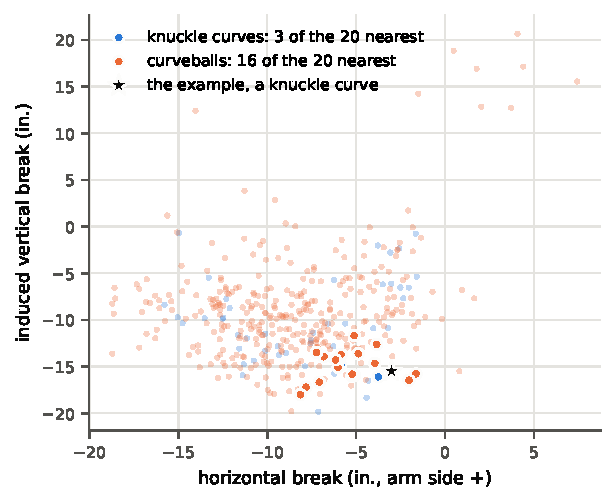
\includegraphics[width=\linewidth]{boundary_neighborhood.pdf}
\caption{The \ExOwnName{} from the example in the text (star) and its 20 nearest pitch shapes from other pitchers in flight space, drawn in the break plane.}\label{fig:neighborhood}
\end{minipage}\hfill
\begin{minipage}[t]{0.44\textwidth}
\centering
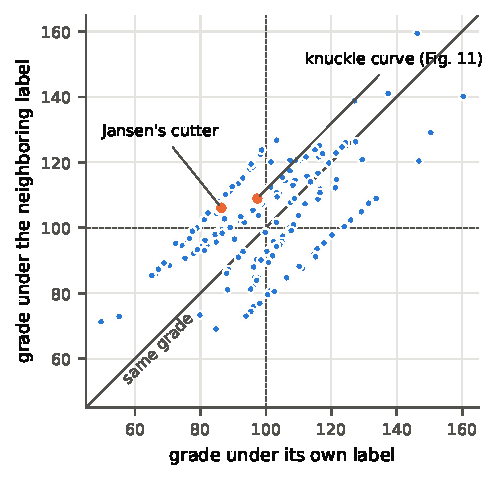
\includegraphics[width=\linewidth]{label_shift.pdf}
\caption{Each 2025 boundary pitch, graded against its own label and against its neighboring label.}\label{fig:labelshift}
\end{minipage}
\end{figure}

In 2026 the effect is replicated, with \LSTwentySixBoundaryPct\% of shapes on a boundary and a median shift of \LSTwentySixShift{} points.
In order to check that this effect does not come only from our model, we also ranked each boundary pitch's actual swinging-strike rate among its own label's pitches and among its neighbor label's pitches, and the two percentiles differ by a median of \LSTwentyFivePctChange{} points in both seasons.
While building this test, we found and removed two artifacts. First, a pitcher's own pitches looked close to each other due to their shared delivery, so we only use other pitchers' shapes as neighbors. Second, absolute velocity made hard changeups look like other pitchers' sinkers, so we use relative velocity instead.

The claim concerns grading \emph{within} a label, as per-type scales and any ``elite among sliders'' comparison do.

\subsection{Where the Lines Fall}
\begin{figure}[tb]
\centering
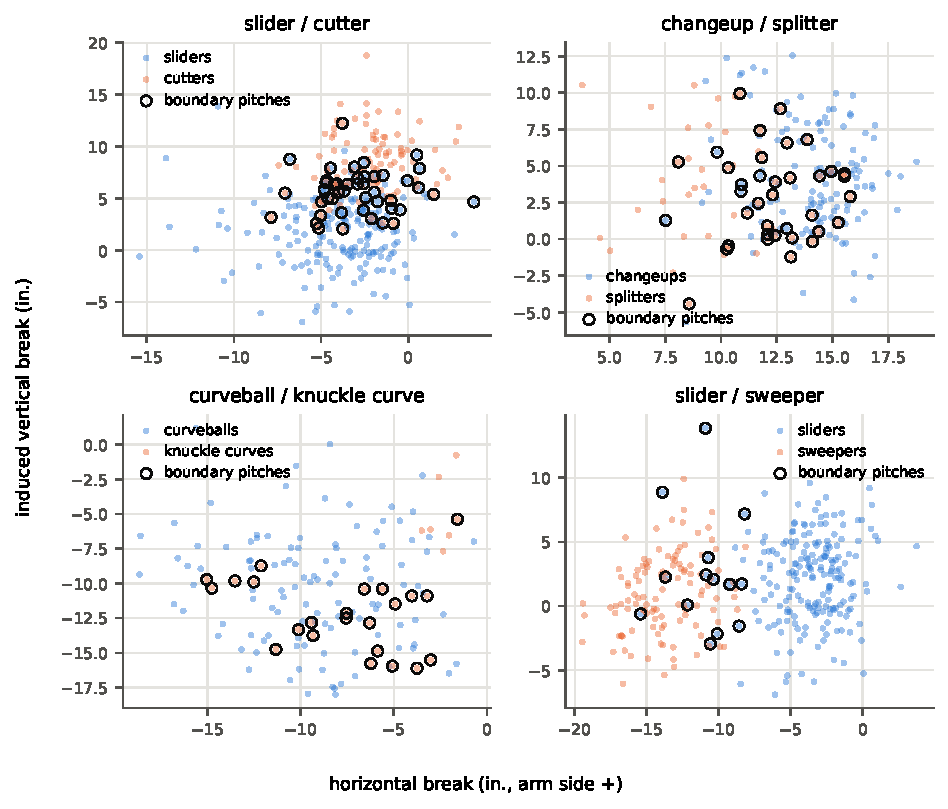
\includegraphics[width=0.78\textwidth]{label_seams.pdf}
\caption{The four most common boundary pairs in 2025 in the break plane, with pitch shapes colored by label and boundary pitches circled.}\label{fig:seams}
\end{figure}
The most common boundary pairs in 2025 are slider and cutter (SL/FC, \LSPairFCSL{} boundary pitches), changeup and splitter (CH/FS, \LSPairCHFS), curveball and knuckle curve (CU/KC, \LSPairCUKC), and slider and sweeper (SL/ST, \LSPairSLST), shown in Figure~\ref{fig:seams}.
Each pair is a place where the geometry and the naming conventions get noisy.
The slider and sweeper pair is the clearest case, since, by definition, a sweeper is a slider with a large amount of horizontal break \parencite{mlbglossary_sweeper}, so the line between them is drawn along one continuous direction of the space. The sweeper label is a more recent addition to Statcast, only being added in 2023.
Statcast's own slurve label makes the same point from the other side, as it names a breaking ball that cannot be clearly defined as a slider or curveball \parencite{mlbglossary_slurve}. 
Many of the observations we make in this paper are well known, but the continuum shows that they are not just a matter of naming conventions, they are a matter of geometry.

For the other three pairs, which pitchers often tell apart by grip as much as by flight, the boundary pitches show that the two labels overlap in flight, as a shape contains close neighbors of both kinds, just as Figure~\ref{fig:neighborhood} shows for a knuckle curve.
Cutters and four-seamers meet the same way, just less often, with \LSPairFCFF{} boundary pitches.
Kenley Jansen's iconic cutter carries the ride of a four-seamer, \JansenNbFF{} of its 20 nearest shapes from other pitchers are four-seamers.
It grades \JansenOwnGrade{} among cutters but \JansenAltGrade{} among four-seamers (Figure~\ref{fig:labelshift}), showing that a simple bucketing can misrepresent a pitch's quality.

\subsection{Thinking Continuously}
The rest of this section is about possibilities rather than results, ideas that the continuum suggests and that we leave to future work.
The Mapper graph is a useful companion here, since it works like a subway map of pitch-shape space, with nodes for neighborhoods of similar pitches and edges where those neighborhoods overlap.
It drops the exact coordinates but shows which regions connect, and the tests of Section~\ref{sec:certify} are what let us trust it.

\subsubsection{Pitch Design and Player Development}
If pitch shapes form one connected space, then any pitch has realistic nearby shapes that other pitchers already throw, and a Stuff+-style grade can tell us which of them grade better.
Although the continuum shows that there are nearby shapes to compare with, and the Mapper graph can suggest which ones, neither knows what a given pitcher can physically throw, since not everyone can throw 100 miles per hour after all.
Which of those shapes to move toward depends on the goal of the design session, so suppose the goal is more swings and misses on a fastball.

As an illustration, we took one veteran's 2025 four-seam fastball and found the \DesignNeighbors{} shapes from other pitchers with nearly the same delivery, velocity, spin rate, and movement.
The pitch is last among them both in our Stuff+-style grade, here put on one scale across all pitch types since the neighbors carry different labels, and in actual swinging-strike rate (\DesignSwStr\%, against a median of \DesignNbSwStr\% for the neighbors), and the better-scoring neighbors have about \DesignIVBGain{} more inches of induced vertical break at nearly the same velocity, so for this goal the reasonable step is more ride.
A pitcher who will not miss many bats might want more ground balls instead, and ranking the same neighborhood by ground-ball rate could point the other way, toward less ride.
Matching the delivery and velocity is what keeps these neighbors within the pitcher's reach, which the Mapper graph alone could not do.

This is an illustration and not a recommendation. The comparison is not causal, our model is a baseline, and a pitch's results also depend on location, sequencing, and deception, which a shape does not capture.

The same idea could start before a pitcher reaches the majors.
Since \textcite{maloof2026classify} find the same three peaks in college pitches that we find in the majors, an amateur's pitch could be placed among major league shapes, and its neighbors within that pitcher's physical limits would project what the pitch could realistically become in a pro development system, whatever it is called today.

\subsubsection{Player Evaluation}
When one pitcher throws two differently labeled pitches that sit in the same region of the space, the two may not be as distinct as their names suggest, which is worth a conversation about how varied that pitcher's repertoire really is.
A key example of this is the four-seam fastball and sinker, where a pitcher may carry two labels, but the shapes may sit close enough that the pitcher is better described as having one fastball with a range of movement.
In pro scouting and acquisition, the same neighborhoods could flag pitchers with upside, since a pitch that grades well below the reachable shapes around it marks a gain that the right development might unlock, and a team could acquire that pitcher before the change rather than after it.

Tunneling makes evaluation a question about pairs as well as single pitches, since two pitches that look alike at the tunnel point and split apart afterward can play off each other even when their shape varies \parencite{sayre2017tunnels}.
Statcast records each pitch's velocity and acceleration 50 feet from home plate \parencite{savantcsvdocs}, so a pitch's position at the tunnel point can be estimated, and one could look for Mapper nodes, or neighborhoods of nodes, whose pitches tunnel well with those of another.
Because tunneling depends on a pitcher's own release point, these pairs would have to be measured within each pitcher and then gathered by region, and whether well-tunneled pairs earn more swings and misses would have to be tested rather than assumed.
But regardless, the Mapper output combined with the tunnel point could suggest which pitches to pair together, and which to avoid pairing, or reasonable additions to a pitcher's arsenal.

\subsubsection{Rethinking Pitch Labels and Grades}
A grade on a per-type scale answers one question, which is how good a pitch is among pitches with the same label.
The continuum suggests a slew of other options, from small changes to large ones.
The smallest is to report a per-type grade along with its label sensitivity, so a reader knows when the label line matters. For boundary pitches, the grade could be reported as a range, from the pitch's grade among its own label to its grade among its neighbors' label.
Next, a pitch could be graded within its family, the grouping the data support most clearly, or against its nearest neighbors in pitch-shape space, so that the comparison group follows the geometry rather than the name.
And as an extreme, a pitch could carry shares of surrounding labels rather than a single name, much as the \ExOwnName{} of Figure~\ref{fig:neighborhood} is mostly \ExAltName{} by its neighbors.

Ultimately, the bigger change may be in how grades are built and labels used.
If grades are to use groups at all, and pitch shape alone gives none beyond the three families, then the groups may have to come from somewhere else, such as how a particular pitch is used, as an example.
Our own grade weights contact, misses, and chases equally for every pitch, as if every pitch had the same job.
Instead, a pitch could first be classified by its role in the arsenal, such as a primary fastball, a ``ground ball pitch'' that limits hard contact, or a putaway pitch, using its usage along with pitch results possibly including but not limited to swinging-strike rate, in-zone whiff rate, chase rate, and quality of contact.
It could then be graded against its shape neighbors within that role, on the outcome that matches the role.
For example, Jansen throws the cutter far more than any other pitch, so it would be graded among other primary pitches, which fits its four-seam neighbors.
Density peaks in role space would show whether such roles are real groups or another continuum, and since roles are partly found from results, a role-based grade would need to be checked on a later season.

Pitch labels are not going away, and they should not, since they give players, coaches, and broadcasters a shared language for the game.
Our results suggest treating them as names for regions of a continuum.
None of the ideas in this section has been tested here, but each starts from the same question, which is where a pitch sits and what is around it.
The goal is not to replace labels, but to use the continuum to make them more informative, and to make pitch grades more robust and more useful for pitch design, player development, and evaluation.

%======================================================================
\section{Discussion and Conclusions}\label{sec:discussion}
%======================================================================
\subsection{Comparison with Prior Work}\label{sec:prior}
Several studies have already grouped pitches by their physical characteristics alone.
\textcite{pane2013trouble} classify PITCHf/x pitches with a Gaussian mixture, and \textcite{camp2020clustering} use $k$-means to find subtypes within the Statcast pitch types, which subdivides the labels without ever testing them.
Closest to our work is \textcite{maloof2026classify}, a non-peer-reviewed article that applies persistent homology to the density of 4.47 million NCAA Division I pitches.
They find three dominant peaks, those being fastball, breaking ball, and changeup, and conclude that finer pitch names are locations along continuous ridges.
As we saw in Section~\ref{sec:peaks}, our results agree with theirs at the level of density peaks, even though we used Major League data and nine coordinates including spin and release.
Our shape results, on the other hand, come from different methods, namely Mapper and its nerve, Vietoris--Rips persistence, and null models.
We did not test their ridge conclusion, but it is consistent with our picture.

Others have raised concerns about reading too much into Mapper's output.
\textcite{topaz2026null} finds that four published Mapper analyses do not exceed a covariance-matched Gaussian null, and in our case the nulls also reproduce the velocity ordering and the slider--cutter band (Section~\ref{sec:shape}).
\textcite{carrieremicheloudot2018} show that Mapper depends heavily on its cover parameters and propose a principled way to choose them, which we see as an alternative to our grid search, and \textcite{vejdemojohansson2018certified} propose tests for whether a cover meets the requirements of the nerve theorem.

\subsection{Limitations}\label{sec:limits}
In general, our results come with a few limitations.
The nine-coordinate shape results only use one season, although the flight-space check (Table~\ref{tab:flight}) and the label-sensitivity results replicate in 2026.
The fit applies no minimum pitch count and keeps slow pitches, both deliberately, since slow curves and shapes with few pitches can still be informative.
While the Mapper features survive minimums of 10 and 20 (Appendix~\ref{app:thin}), we did not rerun persistent homology with a minimum.
We also compare persistence diagrams with null models instead of computing formal confidence sets, and our persistence cutoffs are conventions.
Our null comparisons use few replicates, 10 per lens for stability and 5 for the nerve and persistent homology, so a result above the whole null range is suggestive rather than a formal test, and more replicates would sharpen it.
Our shapes average a pitcher's pitches of each type, which hides the scatter within a shape, and this is the reason we check the dense regions separately at the pitch level.
Finally, the Stuff+-style models are our own reimplementation and methodology and have not been published. We will concede that there are many ways to build a Stuff+ model, and we do not claim that ours is the best, but it is sufficient to illustrate the consequences of a discrete label.

\subsection{Future Studies}
Ultimately, the ideas of Section~\ref{sec:consequences} are baseball questions that still need to be tested on the field, so the next steps we list here are about the mathematics and the data behind them.
Several of our limitations point to their own next steps.
Formal confidence sets for persistence diagrams \parencite{fasy2014confidence} would replace our cutoff conventions, and the principled cover selection of \textcite{carrieremicheloudot2018} would replace our grid search.
The loose end in flight space could be revisited with more seasons, since its loop sits right at our cutoff in both seasons we have.
Since our shapes are averages, running Mapper on single pitches rather than shapes would show whether the continuum holds for the pitches themselves.

The coordinates themselves are another direction.
Movement could also be measured relative to the pitcher's arm slot or release point, and in order to do this, we would need to redesign the coordinates and not just add a column.
Chris Sale serves as a good example, since his release point is far from the average, and measuring movement relative to the average would misrepresent his pitches.
Biomechanical markers, such as pronation and supination, are not recorded by Statcast, but adding them would tie shapes to how pitchers produce them.
Finally, we could repeat the analysis at other levels, such as minor league or college baseball, and follow how pitches change across seasons, which would show how pitchers move through the space as they develop.

\subsection{Conclusion}\label{sec:conclusion}
We set out to ask whether pitch labels mark separate groups or divide one connected space, and the answer is in between, one connected space with a few dense regions that the labels divide.
Apart from the very slow, outlier pitches, pitch shapes form one continuum, with no more gaps or loops than a Gaussian null, and single pitches pile up in three dense regions, those being fastballs, breaking balls, and offspeed pitches.

For the mathematician, the lesson is in how we got there.
At face value, the Mapper graph suggested \GraphBone{} loops, a velocity ladder, and a slider--cutter band, but the full nerve keeps only \NerveBone{} loop, and covariance-matched nulls reproduce the ordering and the band.
Mapper gives us a picture worth looking at, while homology and null models are what tell us which parts of it to believe.

For the baseball reader, the lesson here is that pitch labels are names for regions of a continuum and not natural groupings.
As we saw, grading a pitch within its label is fragile for roughly a tenth of the shapes with enough pitches to test, the ones near a boundary, so we argue that a pitch is better described by where it sits and what is around it, and not only by its name.
Like red and orange, a slider and a cutter are names for places on a continuum, and the line between them is ours to draw.

When we are thinking of pitches as a continuum, we can ask new questions about how to evaluate and design them, and the Mapper graph is a useful companion for that. To fittingly quote Peter Brand in \emph{Moneyball}, it ``opens up all kinds of interesting possibilities.''

%======================================================================
\Needspace{10\baselineskip}
\section*{Acknowledgments}
%======================================================================
I would like to thank my advisor, Dr. Caleb Eckhardt, for his guidance and support throughout this project, and for giving me the freedom to follow my own interests.
I would also like to thank my defense committee members, Dr. Dan Farley and Dr. Louis DeBiasio, whose teaching and passion for topological data analysis and graph theory, respectively, shaped much of this work.
I am grateful to the Department of Mathematics and to Miami University as a whole for the opportunities they have given me to pursue my academic interests and how they intersect with my passion for sports analytics.
Finally, I could not write this section without thanking my family and friends for their support throughout my entire academic journey.

\appendix
\section{Parameters and Reproducibility}\label{app:repro}
\begin{table}[htbp]
\centering
\begin{tabular}{ll}
\toprule
Component & Setting \\
\midrule
Lens & PCA, 2 components (alternatives: velocity $\times$ IVB, Isomap, density) \\
Cover & 10 intervals per axis, 30\% overlap (grid: 8/10/12, 20/30/40\%) \\
Clustering & DBSCAN, $\varepsilon = 1.0$, $M = 4$ (grid: $\varepsilon$ = 0.8/1.0/1.2) \\
Stability & 30 refits on 80\% of pitchers without replacement \\
Null models & Gaussian; within-type shuffle; spin-pair shuffle (flight space) \\
Null replicates & 10 per null and lens (stability); 5 (nerve, persistent homology); \\
 & 50 (density peaks) \\
Persistent homology & Vietoris--Rips; $H_0$ on all shapes, $H_1$ on five 1{,}000-shape subsamples \\
Density peaks & $50^3$ grid, $\sigma = 1$ cell, 50 Gaussian replicates \\
 & grid range: break $\pm 25$ in., relative speed $-25$ to 5 mph \\
Persistence cutoffs & $u$ = median $H_0$ death; long-lived bar $3u$; persistent loop $2u$ \\
Velocity ordering & Spearman $\rho \ge 0.7$ (Definition~\ref{def:features}) \\
Boundary pitches & at least 150 pitches; 20 nearest other-pitcher shapes in flight space, \\
 & relative velocity; at least half carry one other label \\
Stuff+-style models & CatBoost, trained 2022--24, five-fold out-of-fold; xwOBA, \\
 & swinging strike, and chase, with equal weights \\
Pitch-design neighbors & release within 0.5 ft, velocity within 1.5 mph, spin within 200 rpm, \\
 & movement within 4 in. \\
\bottomrule
\end{tabular}
\caption{Parameters of every analysis in the paper.}\label{tab:params}
\end{table}
Table~\ref{tab:params} lists the parameters of every analysis. Code and data products are at \url{https://github.com/WillPaz16/tda-pitch-clustering}. Every computed result in this paper is generated from saved outputs by \nolinkurl{src/viz/paper_numbers.py}, and every figure by \nolinkurl{src/viz/thesis_figures.py}.

\section{Minimum Pitch Counts}\label{app:thin}
Table~\ref{tab:thin} repeats the main Mapper fit with a minimum number of pitches per shape.
The table rebuilds the shapes from a later download, and Statcast revises some pitch labels after the fact, so a minimum of 1 gives \SSOneShapes{} shapes rather than \NShapes.
The velocity ordering is unaffected. Slow shapes stay outside the largest component, but at a minimum of 20 they are too few to form clusters of their own.

\begin{table}[!htbp]
\centering
\begin{tabular}{rrrrcc}
\toprule
Min.\ pitches & Shapes & Slow shapes & Components & Slow isolated & Ordering $\rho$ \\
\midrule
1 & \SSOneShapes & \SSOneSlow & \SSOneComp & \SSOneIso & \SSOneRho \\
10 & \SSTenShapes & \SSTenSlow & \SSTenComp & \SSTenIso & \SSTenRho \\
20 & \SSTwentyShapes & \SSTwentySlow & \SSTwentyComp & \SSTwentyIso & \SSTwentyRho \\
\bottomrule
\end{tabular}
\caption{The main Mapper fit with a minimum pitch count per shape. ``Slow isolated'' is the share of slow shapes lying only outside the largest component, and ``Ordering $\rho$'' is the velocity ordering of Definition~\ref{def:features}.}\label{tab:thin}
\end{table}

\section{Use of AI Assistance}
This project was developed with help from Claude, Anthropic's AI assistant, used through Claude Code, which assisted with analysis code, documentation, the literature search, and outlining.
The author set the research questions and scope, made the methodological decisions, and reviewed all results from the code outputs.
Because AI output can be confidently wrong, the work was built around verification. Every structural claim is tested against null models and across parameters, subsamples, and lenses before it counts as a finding. 
Much of the coding was initially done by Claude Code, but the work was double-checked by the author ensuring to read each individual output.
In regard to literature review, Claude was used to locate citations rather than learn the information for the author.
A citation is used only after it was reviewed and read by the author to ensure validity. 
For outlining, based on the work and desired narrative, Claude helped draft and outline this document as a starting point for the author to write.

\printbibliography

\end{document}
